\chapter{Testare și validare}\label{ch:testare}
\pagestyle{fancy}

Capitolul prezintă rezultatele experimentale obținute și, înaintea lor, verificările care garantează că aceste rezultate măsoară ceea ce își propun să măsoare. Ordinea este deliberată: o rată de evaziune are sens doar dacă lanțul care a produs-o a fost validat în prealabil. Sunt raportate, în ordine, metodologia de testare, validarea lanțului de prelucrare, performanța clasificatoarelor pe trafic nemodificat, rezultatele măsurării evaziunii și analiza de sensibilitate.

\section{Metodologia de testare}\label{sec:metodologie}

\subsection{Mediul experimental}\label{subsec:mediu}

Experimentele au fost executate pe o singură configurație, cu versiuni fixate ale tuturor bibliotecilor, înregistrate automat la fiecare rulare în fișierul de metadate descris în secțiunea~\ref{sec:reproductibilitate}. Antrenarea rețelei neuronale a folosit accelerare grafică, iar restul etapelor se execută pe procesor.

Setul de date este utilizat în partiția oficială, fără reeșantionare și fără eliminarea vreunei observații. Partiția de testare conține 82\,332 de înregistrări, dintre care 45\,332 corespund traficului malițios. Toate măsurătorile adversariale se raportează exclusiv la aceste 45\,332 de fluxuri, filtrate ulterior prin criteriul de eligibilitate subsecțiunea~\ref{subsec:eligibil}.

\subsection{Nivelurile de verificare}\label{subsec:niveluri}

Testarea este organizată pe patru niveluri, fiecare adresând o clasă distinctă de erori:

\begin{enumerate}
    \item \textbf{Determinismul} (\textit{determinism}): aceeași intrare produce aceeași ieșire între rulări repetate.
    \item \textbf{Validitatea variantelor} (\textit{validity}): fiecare variantă perturbată respectă constrângerile din subsecțiunea~\ref{subsec:admisibile}.
    \item \textbf{Capacitatea de respingere} (\textit{negative testing}): suita de validare respinge efectiv variante invalide construite intenționat.
    \item \textbf{Invarianții de capăt la capăt} (\textit{end-to-end invariants}): varianta identică reproduce predicțiile de referință și produce evaziune nulă.
\end{enumerate}


\section{Caracterizarea setului de date}\label{sec:caracterizare}

\subsection{Distribuția claselor}\label{subsec:distributie}

Tabelul~\ref{tab:distributie} prezintă distribuția claselor în partiția de antrenare.

\begin{table}[!ht]
    \caption{Distribuția claselor în partiția de antrenare}
    \centering
    \begin{tabular}{|l|r|r|}
        \hline
        \textbf{Clasă} & \textbf{Observații} & \textbf{Pondere} \\
        \hline
        Normal & 56\,000 & 31,9\% \\
        \hline
        Generic & 40\,000 & 22,8\% \\
        \hline
        Exploits & 33\,393 & 19,0\% \\
        \hline
        Fuzzers & 18\,184 & 10,4\% \\
        \hline
        DoS & 12\,264 & 7,0\% \\
        \hline
        Reconnaissance & 10\,491 & 6,0\% \\
        \hline
        Analysis & 2\,000 & 1,1\% \\
        \hline
        Backdoor & 1\,746 & 1,0\% \\
        \hline
        Shellcode & 1\,133 & 0,6\% \\
        \hline
        Worms & 130 & 0,07\% \\
        \hline
    \end{tabular}
    \label{tab:distributie}
\end{table}

Raportul dintre clasa cea mai frecventă și cea mai rară este de \textbf{431 la 1}. Un asemenea dezechilibru confirmă inadecvarea acurateței globale ca indicator, discutată în secțiunea~\ref{sec:metrici}: un clasificator care ar prezice constant clasa majoritară ar obține o acuratețe de aproape $32\%$ fără nicio capacitate de discriminare, iar clasa cea mai rară ar putea fi ratată complet cu un cost neglijabil în acuratețe. Distribuția este reprezentată grafic, pe scară logaritmică, în figura~\ref{fig:distributie}.

\begin{figure}[!ht]
    \centering
    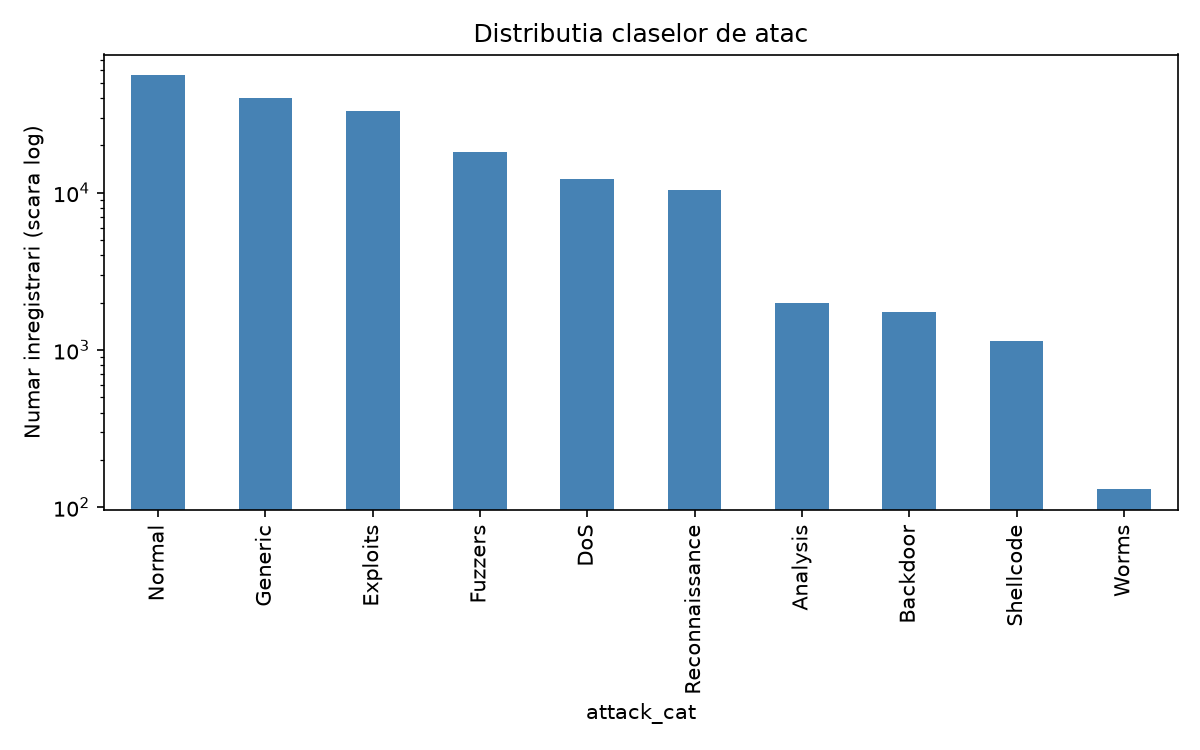
\includegraphics[width=0.85\textwidth]{figs/eda_class_distribution.png}
    \caption{Distribuția celor zece clase în partiția oficială de antrenare a setului UNSW-NB15, cele 175\,341 de fluxuri. Scara verticală este logaritmică, întrucât raportul dintre clasa cea mai frecventă și cea mai rară depășește $430{:}1$, iar pe scară liniară toate clasele rare ar fi indistinctibile de axă.}
    \label{fig:distributie}
\end{figure}

\subsection{Variabilele categorice}\label{subsec:categorice}

Analiza cardinalității variabilelor categorice a condus la două constatări cu efect direct asupra preprocesării.

Variabila care descrie protocolul are 133 de valori distincte, dintre care primele două acoperă împreună peste jumătate din observații, iar 118 apar de mai puțin de 200 de ori. La pragul de 50 de apariții folosit de mecanismul de grupare descris în subsecțiunea~\ref{subsec:rare}, doar trei protocoale sunt colapsate, ceea ce confirmă că reducerea dimensionalității nu este beneficiul principal al mecanismului în acest set.

Variabila care descrie starea conexiunii conține două valori prezente exclusiv în partiția de testare. Această situație justifică menținerea grupării: fără ea, valorile respective ar fi tratate tăcut, fără nicio urmă în raportare.

Variabila care descrie serviciul are o particularitate proprie: valoarea rezervată pentru serviciu necunoscut acoperă aproximativ 54\% din observații. Ea nu este, prin urmare, o categorie în sens obișnuit, ci un indicator de absență a informației.

\subsection{Caracteristicile numerice}\label{subsec:numerice}

Distribuțiile numerice sunt puternic asimetrice, cu coeficienți de asimetrie care ating valoarea 167 pentru adâncimea tranzacției și depășesc 39 pentru volumele de octeți și numărul de pachete. Asimetria justifică utilizarea scării logaritmice la reprezentarea grafică, dar nu impune nicio transformare în fluxul de modelare, din motivele expuse în subsecțiunea~\ref{subsec:eda}.

Analiza corelațiilor cu eticheta produce constatarea care se dovedește centrală pentru întreaga lucrare: valoarea TTL a pachetelor emise are coeficientul de corelație cel mai ridicat din întregul set, $0{,}693$, urmată de contorul de context asociat, cu $0{,}578$. Nicio altă caracteristică nu depășește valoarea $0{,}40$ în modul.

Primele două poziții sunt ocupate de o caracteristică asociată valorii TTL și de o caracteristică derivată din aceasta. Importanța lor ridicată sugerează încă din analiza exploratorie că modificarea acestor caracteristici poate influența predicțiile modelului, aspect evaluat ulterior în secțiunea~\ref{sec:rezultate-o3}. Verificarea setului de date nu a evidențiat valori lipsă, coloane cu varianță nulă sau înregistrări duplicate.


\section{Validarea lanțului de prelucrare}\label{sec:validare-lant}

\subsection{Verificarea determinismului}\label{subsec:det}

Instabilitatea predicției modelului Random Forest, descrisă în subsecțiunea~\ref{subsec:inferenta}, a fost măsurată direct înainte de corectare. Cinci apeluri identice de predicție pe același set de intrare au produs, față de o referință stocată, un număr de nepotriviri de $0, 1, 0, 1, 0$, variație mică în valoare absolută, dar nenulă și nedeterministă.

După impunerea execuției pe un singur fir, verificarea a fost repetată pe zece rulări consecutive, cu zero nepotriviri în toate cazurile. S-a confirmat totodată că predicțiile obținute în regim determinist coincid integral cu cele stocate anterior, ceea ce arată că măsura elimină variabilitatea fără a modifica vreun rezultat.

Au fost identificate 44 de fluxuri aflate în situația critică: 43 la egalitate exactă între primele două clase și unul cu o diferență la limita preciziei de reprezentare. Într-un set în care clasa cea mai rară are 44 de observații în partiția de testare, un asemenea număr de comutări posibile nu poate fi tratat ca zgomot.

\subsection{Validarea variantelor perturbate}\label{subsec:valvar}

Cele 28 de variante generate au fost supuse integral componentei de verificare din tabelul~\ref{tab:verificari}. Rezultatul este prezentat în tabelul~\ref{tab:validitate}.

\begin{table}[!ht]
    \caption{Rezultatul validării variantelor perturbate}
    \centering
    \begin{tabular}{|l|c|}
        \hline
        \textbf{Mărime} & \textbf{Valoare} \\
        \hline
        Fluxuri de atac prelucrate & 45\,332 \\
        \hline
        Variante generate & 28 \\
        \hline
        Verificări executate & 1\,259 \\
        \hline
        Verificări eșuate & \textbf{0} \\
        \hline
        Nepotriviri pe varianta identică & \textbf{0} \\
        \hline
    \end{tabular}
    \label{tab:validitate}
\end{table}

Creșterea maximă a erorii relative a identităților algebraice, măsurată per rând pe toate cele 28 de variante, a fost de ordinul $10^{-15}$, adică la nivelul preciziei de reprezentare în virgulă mobilă. Propagarea prin rapoarte, enunțată în subsecțiunea~\ref{subsec:propagare}, se comportă, prin urmare, exact conform predicției teoretice: ea nu degradează consistența internă a vectorului.

\subsection{Testarea negativă a suitei de validare}\label{subsec:negativ}

Pentru a demonstra că suita este capabilă să respingă, au fost construite șapte variante deliberat invalide, fiecare încălcând o singură constrângere. Rezultatele sunt prezentate în tabelul~\ref{tab:negativ}.

\begin{table}[!ht]
    \caption{Testarea negativă: variante invalide construite intenționat}
    \centering
    \begin{tabular}{|p{6.4cm}|l|}
        \hline
        \textbf{Încălcare introdusă} & \textbf{Rezultat} \\
        \hline
        Umplutură aplicată în sens invers & Respinsă \\
        \hline
        Durată redusă în loc de dilatată & Respinsă \\
        \hline
        Contor de conexiuni crescut & Respinsă \\
        \hline
        Coloană generată de victimă modificată & Respinsă \\
        \hline
        Caracteristică identitară rescrisă & Respinsă \\
        \hline
        Valoare nedefinită injectată prin propagare & Respinsă \\
        \hline
        Schemă alterată (tip de dată modificat) & Respinsă \\
        \hline
    \end{tabular}
    \label{tab:negativ}
\end{table}

Toate cele șapte variante au fost respinse, fiecare de verificarea corespunzătoare încălcării introduse. Rezultatul confirmă că cele 1\,259 de verificări trecute din tabelul~\ref{tab:validitate} constituie o dovadă de validitate, nu doar o execuție fără eroare.

Această etapă a avut și un rol corectiv. În versiunile intermediare, două verificări treceau din motive greșite: cea de consistență a dependențelor, din cauza unei toleranțe calculate global, și cea de limite de domeniu, din cauza unor praguri absolute. Ambele au fost descoperite exclusiv prin testare negativă și au fost reformulate conform discuției din subsecțiunea~\ref{subsec:validare}.

\subsection{Verificarea variantei nemodificate}
\label{subsec:invidentitate}

Varianta de nivel zero nu modifică valorile fluxurilor, dar trece prin toate etapele procesului de evaluare: generare, propagare, restabilirea tipurilor de date, validare și predicție. Scopul acestei verificări este de a determina dacă prelucrarea datelor produce modificări neintenționate.

Predicțiile obținute după prelucrare au fost comparate cu cele calculate direct pe fluxurile originale. Verificarea a fost realizată pentru toate cele trei modele și pentru cele 45\,332 de fluxuri de atac. Nu a fost identificată nicio diferență între predicții.

Rezultatul arată că trecerea datelor prin procesul de evaluare nu modifică predicțiile atunci când perturbarea este nulă. Verificarea poate evidenția erori precum schimbarea ordinii caracteristicilor, conversia incorectă a tipurilor de date sau actualizarea necorespunzătoare a caracteristicilor derivate.

\subsection{Verificarea montajului de antrenare adversarială}\label{subsec:val-adversarial}

Etapa de antrenare adversarială este singura care produce modele noi. Din acest motiv, este și singura care ar putea introduce o abatere față de rezultatele deja măsurate fără ca aceasta să se vadă în cifrele finale. Înainte de a interpreta vreun rezultat, au fost verificate separat elementele de mai jos.

\textbf{Reproducerea modelelor de referință.} Grupul antrenat pe datele originale ar trebui să fie identic cu modelul înghețat din capitolul anterior, primind exact aceleași date și aceiași hiperparametri. Există totuși o diferență de formă: ponderile de clasă îi sunt date ca listă explicită de valori, în locul cuvântului-cheie prin care biblioteca le calcula singură din numărătorile setului primit. Schimbarea era necesară pentru grupurile augmentate, unde numărătorile diferă, dar trebuia arătat că pe datele originale nu schimbă nimic. Altfel, chiar grupul de referință ar fi fost altul decât modelul înghețat, iar abaterea s-ar fi transmis tăcut tuturor comparațiilor. Comparația s-a făcut rând cu rând, pe întreaga partiție de testare, iar rezultatele sunt prezentate în tabelul~\ref{tab:reproducere}.

\begin{table}[!ht]
    \caption{Reproducerea modelelor înghețate de către grupul de referință}
    \centering
    \begin{tabular}{|l|c|c|}
        \hline
        \textbf{Model} & \textbf{Rânduri comparate} & \textbf{Nepotriviri} \\
        \hline
        Random Forest & 82\,332 & \textbf{0} \\
        \hline
        XGBoost & 82\,332 & \textbf{0} \\
        \hline
        Transformer & 82\,332 & \textbf{0} \\
        \hline
    \end{tabular}
    \label{tab:reproducere}
\end{table}

Pentru Transformer, egalitatea este mai puternică decât o simplă coincidență a predicțiilor finale: valorile funcției de cost și scorurile de validare ale primelor epoci coincid până la a patra zecimală cu cele înregistrate la antrenarea modelului de referință, ceea ce arată că traiectoria de optimizare este identică, nu doar punctul ei final. Rezultatul confirmă că fixarea ponderilor este, pe datele originale, o operație neutră, deci orice diferență observată la celelalte grupuri provine din date.

\textbf{Reproducerea lanțului de măsurare.} Modulul de evaluare al acestei etape parcurge grila de variante printr-un drum de cod propriu, distinct de cel folosit la măsurarea sistematică din secțiunea~\ref{sec:rezultate-o3}. Pentru a exclude o divergență între cele două, modelele înghețate au fost trecute prin noul drum și ratele obținute au fost comparate cu cele deja raportate. Pentru XGBoost, toate cele 28 de variante au coincis exact, cu o diferență absolută maximă de $0{,}0000$ puncte procentuale, iar numărul de fluxuri semnalate a fost identic, 44\,258. Măsurătorile noi sunt, prin urmare, direct comparabile cu cele anterioare.

\textbf{Proveniența statisticilor de generare.} Restricția din subsecțiunea~\ref{subsec:provenienta} a fost verificată prin numărul de combinații din tabelul de corespondențe al contorului de context: contextul construit pe ambele partiții conține 58 de combinații, iar cel construit exclusiv pe partiția de antrenare, 32. Diferența confirmă că restricția este efectivă, nu declarativă. Consecința practică este că generatorul recurge mai des la valorile de rezervă atunci când produce date de antrenare, ceea ce este raportat în fișa rulării.

\textbf{Compoziția seturilor augmentate.} Cu 175\,341 de rânduri în partiția de antrenare, dintre care 119\,341 de atac, adăugarea unei copii per flux malițios produce 294\,682 de rânduri, adică un factor de $1{,}68$, nu de $2$. Raportul dintre traficul de atac și cel normal crește de la $2{,}13$ la $4{,}26$. Grupul de control are, prin construcție, exact aceleași valori: aceeași dimensiune, aceleași numărătoare per clasă, aceeași proporție. Amprentele criptografice ale celor două seturi diferă, ceea ce confirmă că diferă efectiv prin conținut, nu doar prin etichetă.

\textbf{Împărțirea și apartenența la aceeași parte.} Împărțirea în sub-set de antrenare și set de validare coincide, la nivel de identificator, cu cea folosită la antrenarea modelului de referință. Verificarea de apartenență a confirmat că toți cei 149\,039 de identificatori sursă ai rândurilor generate provin din sub-setul de antrenare, niciunul din setul de validare.


\section{Performanța clasificatoarelor pe trafic nemodificat}\label{sec:rezultate-o1}

\subsection{Performanța globală}\label{subsec:global}

Tabelul~\ref{tab:metrici} prezintă rezultatele celor trei modele pe partiția oficială de testare.

\begin{table}[!ht]
    \caption{Performanța modelelor pe traficul nemodificat}
    \centering
    \begin{tabular}{|l|c|c|c|c|}
        \hline
        \textbf{Model} & \textbf{Acuratețe} & \textbf{Acuratețe ech.} & \textbf{Macro-$F1$} & \textbf{$F1$ ponderat} \\
        \hline
        Random Forest & 0,6913 & 0,5944 & 0,5010 & 0,7416 \\
        \hline
        XGBoost & \textbf{0,7659} & 0,5443 & \textbf{0,5098} & \textbf{0,7816} \\
        \hline
        Transformer & 0,6594 & \textbf{0,6288} & 0,4354 & 0,7168 \\
        \hline
    \end{tabular}
    \label{tab:metrici}
\end{table}

Ordinea modelelor depinde de metrica aleasă, ceea ce confirmă necesitatea raportării mai multor indicatori. Modelul cu XGBoost conduce la acuratețe, macro-$F1$ și $F1$ ponderat, în timp ce Transformer obține cea mai bună acuratețe echilibrată, adică cel mai bun comportament mediu pe clase, dar cel mai slab macro-$F1$. Diferența provine din faptul că acuratețea echilibrată mediază sensibilitățile, în timp ce macro-$F1$ penalizează și precizia scăzută: Transformer identifică o proporție mai mare din observațiile claselor rare, dar cu multe alarme false pe acele clase.

Poziția a treia a rețelei la macro-$F1$ nu constituie un eșec, ci rezultatul așteptat. Pe date tabelare, ansamblurile de arbori sunt frecvent competitive sau superioare arhitecturilor neuronale, iar obiectivul comparației, formulat în subsecțiunea~\ref{subsec:comparatie}, nu este stabilirea celui mai performant model, ci observarea comportamentului sub perturbări al unor modele cu predispoziții inductive diferite.

\subsection{Analiza per clasă}\label{subsec:perclasa}

Tabelul~\ref{tab:perclasa} prezintă scorul $F1$ pe fiecare clasă, împreună cu suportul acesteia în partiția de testare.

\begin{table}[!ht]
    \caption{Scorul $F1$ pe clase și suportul acestora în partiția de testare}
    \centering
    \begin{tabular}{|l|r|c|c|c|}
        \hline
        \textbf{Clasă} & \textbf{Suport} & \textbf{RF} & \textbf{XGB} & \textbf{Transformer} \\
        \hline
        Generic & 18\,871 & 0,981 & 0,985 & 0,981 \\
        \hline
        Normal & 37\,000 & 0,766 & 0,847 & 0,738 \\
        \hline
        Reconnaissance & 3\,496 & 0,849 & 0,866 & 0,757 \\
        \hline
        Exploits & 11\,132 & 0,699 & 0,711 & 0,645 \\
        \hline
        Worms & 44 & 0,593 & 0,500 & 0,241 \\
        \hline
        Shellcode & 378 & 0,399 & 0,495 & 0,267 \\
        \hline
        Fuzzers & 6\,062 & 0,376 & 0,396 & 0,355 \\
        \hline
        DoS & 4\,089 & 0,226 & 0,198 & \textbf{0,250} \\
        \hline
        Backdoor & 583 & 0,097 & 0,039 & \textbf{0,116} \\
        \hline
        Analysis & 677 & 0,025 & 0,062 & 0,003 \\
        \hline
    \end{tabular}
    \label{tab:perclasa}
\end{table}

Distribuția scorurilor este puternic neuniformă și se corelează doar parțial cu suportul. Clasa \textit{Generic} este recunoscută aproape perfect de toate modelele, în timp ce clasa \textit{Analysis}, cu un suport comparabil cu al altor clase rezonabil clasificate, este practic ratată de toate trei. Explicația nu este statistică, ci structurală: clasele \textit{Analysis} și \textit{Backdoor} se suprapun aproape complet în spațiul caracteristicilor, iar modelele nu dispun de informația necesară pentru a le separa.

Se observă totodată că Transformer obține cele mai bune scoruri pe \textit{DoS} și \textit{Backdoor}, adică exact pe două dintre clasele cele mai dificile, dar se prăbușește complet pe \textit{Analysis}. Comportamentul este consistent cu acuratețea echilibrată superioară din tabelul~\ref{tab:metrici}.

Matricele de confuzie confirmă interpretarea structurală. Cea a modelului XGBoost este prezentată în figura~\ref{fig:cm-xgb}, iar cea a modelului Random Forest în figura~\ref{fig:cm-rf}. În ambele cazuri, erorile nu sunt distribuite uniform, ci concentrate în blocuri corespunzătoare grupurilor de clase confundabile, ceea ce arată că modelele nu greșesc aleator, ci sistematic, între categorii care se suprapun în spațiul caracteristicilor.

\begin{figure}[!ht]
    \centering
    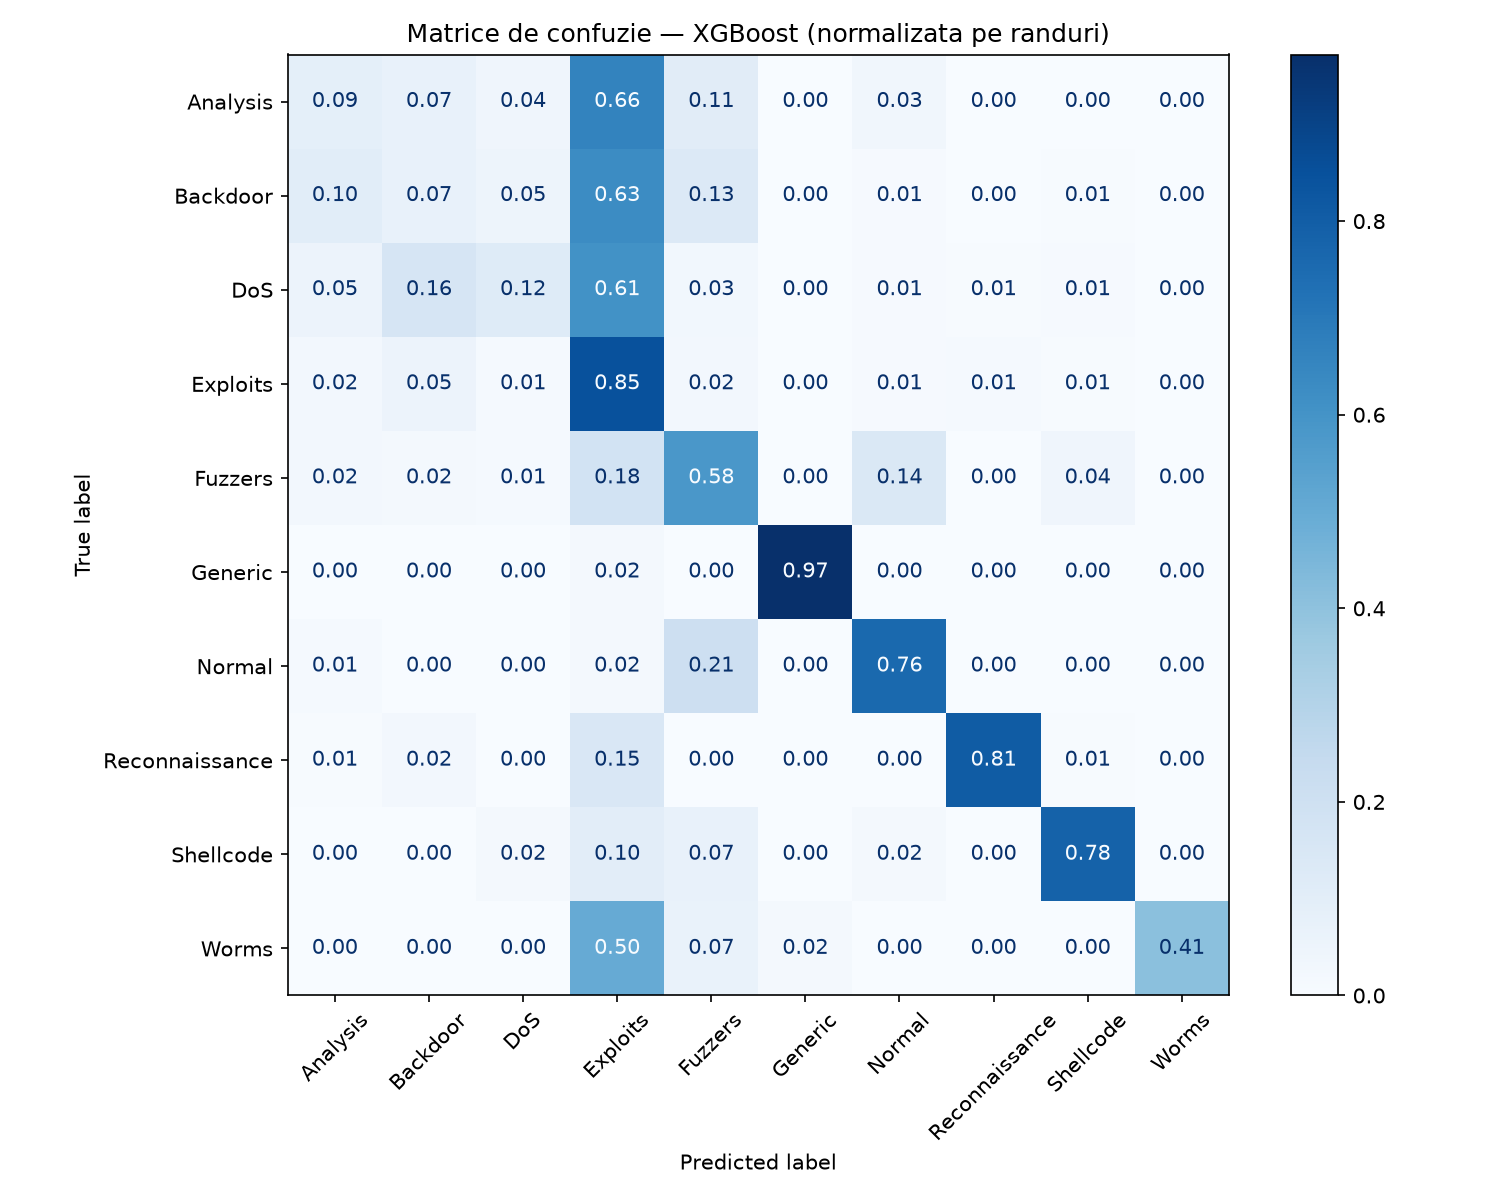
\includegraphics[width=0.80\textwidth]{figs/confusion_matrix_xgboost.png}
    \caption{Matricea de confuzie a modelului XGBoost}
    \label{fig:cm-xgb}
\end{figure}

\begin{figure}[!ht]
    \centering
    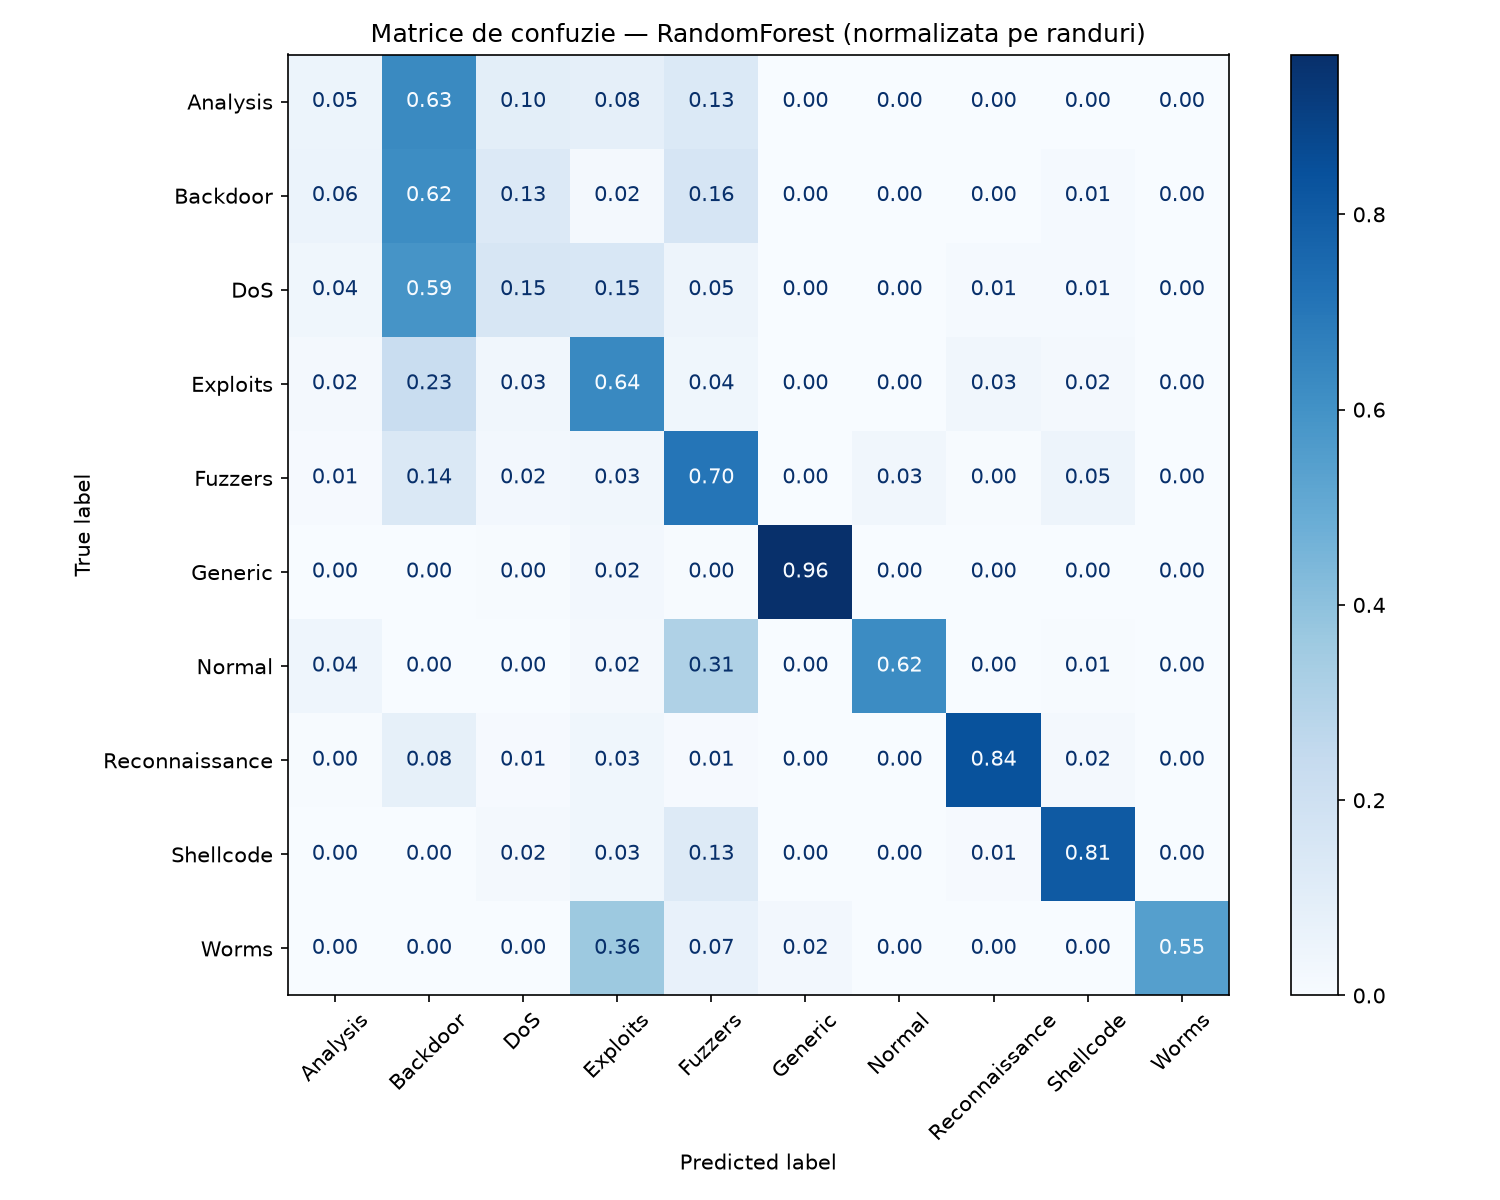
\includegraphics[width=0.80\textwidth]{figs/confusion_matrix_randomforest.png}
    \caption{Matricea de confuzie a modelului Random Forest}
    \label{fig:cm-rf}
\end{figure}

Se observă în ambele matrice că un număr important de fluxuri de atac sunt încadrate în categorii de atac greșite, dar foarte puține sunt clasificate drept trafic legitim. Această asimetrie este exact fenomenul cuantificat în subsecțiunea~\ref{subsec:semnalare}.

\subsection{Capacitatea de semnalare față de acuratețea subtipului}\label{subsec:semnalare}

Rezultatul cel mai important al acestei etape nu apare în tabelul~\ref{tab:metrici}. Deși macro-$F1$ se situează în jurul valorii de $0{,}50$, ceea ce ar sugera o capacitate de detecție modestă, aproape fiecare flux de atac declanșează o alarmă. Decalajul dintre cele două mărimi este prezentat în tabelul~\ref{tab:eligibil}, împreună cu prețul plătit pentru el pe traficul legitim.

\begin{table}[H]
    \caption{Cele două fețe ale detecției pe trafic nemodificat. Primele două coloane se referă la cele 45\,332 de fluxuri de atac, ultima la cele 37\,000 de fluxuri legitime.}
    \centering
    \begin{tabular}{|l|r|r|r|}
        \hline
        \textbf{Model} & \textbf{Clasificate corect} & \textbf{Alarmă declanșată} & \textbf{Alarme false} \\
        \hline
        Random Forest & 33\,812 \;(74,6\%) & \textbf{45\,116 \;(99,52\%)} & 13\,893 \;(37,5\%) \\
        \hline
        XGBoost & 35\,085 \;(77,4\%) & \textbf{44\,258 \;(97,63\%)} & 9\,029 \;(24,4\%) \\
        \hline
        Transformer & 32\,617 \;(72,0\%) & \textbf{45\,304 \;(99,94\%)} & 15\,326 \;(41,4\%) \\
        \hline
    \end{tabular}
    \label{tab:eligibil}
\end{table}

Distanța dintre primele două coloane este substanțială la toate trei modelele: 11\,304 fluxuri la Random Forest, 9\,173 la XGBoost și 12\,687 la Transformer sunt semnalate ca malițioase fără a fi încadrate în categoria corectă. Modelele greșesc mult mai des \emph{care} atac este decât \emph{dacă} este un atac.

A treia coloană arată însă că rata ridicată de semnalare nu trebuie citită ca o performanță de detecție. Modelele semnalează aproape toate atacurile și pentru că semnalează mult prea des în general: între un sfert și peste patru zecimi din traficul legitim primește alarmă. Matricea de confuzie din figura~\ref{fig:cm-rf} arată sursa principală, aproape o treime din traficul legitim fiind încadrat de Random Forest în clasa \textit{Fuzzers}. Un sistem cu acest profil ar fi greu de folosit în practică, unde volumul traficului legitim depășește cu ordine de mărime traficul de atac.

Nivelul acestor rate trebuie însă raportat la partiția pe care sunt măsurate. Partiția oficială UNSW-NB15 este dificilă tocmai pentru că cele două jumătăți ale ei nu provin din aceeași distribuție. Proporția traficului legitim crește de la $31{,}9\%$ la antrenare la $44{,}9\%$ la testare, iar în interiorul clasei legitime ponderea fluxurilor care poartă valoarea TTL 254, cea caracteristică atacurilor, se dublează, de la $20{,}1\%$ la $40{,}7\%$. La testare, modelele întâlnesc prin urmare de două ori mai mult trafic legitim purtând exact semnătura pe care au învățat-o ca indiciu de atac, ceea ce explică direct nivelul alarmelor false. Constatarea nu justifică valorile, dar arată că ele reflectă în bună măsură o proprietate a partiției, nu doar o alegere de model. Ele nu ar trebui, prin urmare, extrapolate ca rate de fals pozitiv ale acestor modele în general.

Constatarea are două consecințe. Prima este că definiția mulțimii eligibile din subsecțiunea~\ref{subsec:eligibil} nu este o convenție lipsită de efect: cele două criterii posibile diferă cu aproape un sfert din observații, iar alegerea între ele modifică numitorul tuturor ratelor raportate ulterior. A doua este că evaziunea devine o măsurătoare netrivială: dacă modelele ar rata deja o fracțiune importantă din atacuri, o rată de evaziune ridicată nu ar demonstra nimic despre efectul perturbării. Punctul de plecare fiind o semnalare cvasicompletă a atacurilor, orice creștere a evaziunii este atribuibilă perturbării. Argumentul se sprijină exclusiv pe coloana a doua din tabel și rămâne valabil indiferent de numărul alarmelor false, întrucât acestea privesc fluxuri legitime, care nu intră în măsurătoare.

\section{Antrenarea modelului Transformer}\label{sec:rezultate-transformer}

Antrenarea a parcurs 44 de epoci înainte de oprirea timpurie, cu selecția modelului la epoca 34 conform criteriului netezit descris în subsecțiunea~\ref{subsec:retea}. Curba scorului de validare a crescut rapid în primele epoci, după care a oscilat în jurul unui platou, ceea ce indică o convergență reală, nu un buget de antrenare insuficient.

Necesitatea criteriului netezit a fost confirmată empiric. Selecția pe valoarea instantanee a scorului de validare indica drept optim un maxim izolat, situat cu peste două abateri standard deasupra mediei locale a traiectoriei și urmat imediat de o revenire la nivelul anterior, adică semnătura tipică a unei fluctuații, nu a unui optim. Criteriul netezit, aplicat pe o fereastră de trei epoci, selectează în schimb un punct dintr-o regiune stabilă.

Este de subliniat că trecerea la criteriul netezit \emph{nu} a îmbunătățit scorul final: macro-$F1$ a scăzut ușor față de selecția pe valoarea instantanee, cu o diferență inferioară amplitudinii oscilațiilor de la o epocă la alta, ceea ce face cele două variante indistinctibile statistic. Justificarea păstrării criteriului netezit este metodologică, nu numerică: modelul reținut este reprezentativ pentru o regiune stabilă a traiectoriei, ceea ce constituie cerința corectă pentru un model destinat unor experimente ulterioare.

\section{Măsurarea ratei de evaziune}\label{sec:rezultate-o3}

\subsection{Rezultatul principal}\label{subsec:principal}

Tabelul~\ref{tab:evaziune} prezintă ratele de evaziune la intensitatea maximă a fiecărui tip de transformare realizabilă. Pentru transformările care implică valori TTL, rezultatul este raportat ca interval, conform discuției din subsecțiunea~\ref{subsec:interval}.

\begin{table}[!ht]
    \caption{Rate de evaziune la intensitate maximă (\% din fluxurile eligibile)}
    \centering
    \begin{tabular}{|l|c|c|c|}
        \hline
        \textbf{Transformare} & \textbf{RF} & \textbf{XGB} & \textbf{Transformer} \\
        \hline
        TTL & 4,4 -- 18,4 & \textbf{50,2 -- 51,1} & 4,0 -- 43,2 \\
        \hline
        Combinată & 31,3 -- 75,9 & \textbf{96,4 -- 96,9} & 17,4 -- 71,0 \\
        \hline
        Umplutură & 0,15 & 1,23 & 0,10 \\
        \hline
        Temporizare & 0,73 & 1,12 & 0,02 \\
        \hline
        Rată conexiuni & 0,33 & 0,56 & 0,00 \\
        \hline
    \end{tabular}
    \label{tab:evaziune}
\end{table}

\medskip
Rezultatul central este net: \textbf{modificarea TTL este singurul vector de perturbare care contează}. Umplutura, dilatarea temporală și reducerea ratei de conexiuni lasă rata de evaziune sub $1{,}3\%$ la orice intensitate și pentru orice model, în timp ce o singură modificare a valorii TTL duce XGBoost de la $0\%$ la peste $50\%$. Combinată cu celelalte transformări, aceeași modificare împinge rata la aproape $97\%$.

Evoluția pe niveluri de intensitate este prezentată în figura~\ref{fig:curbe}.

\begin{figure}[H]
    \centering
    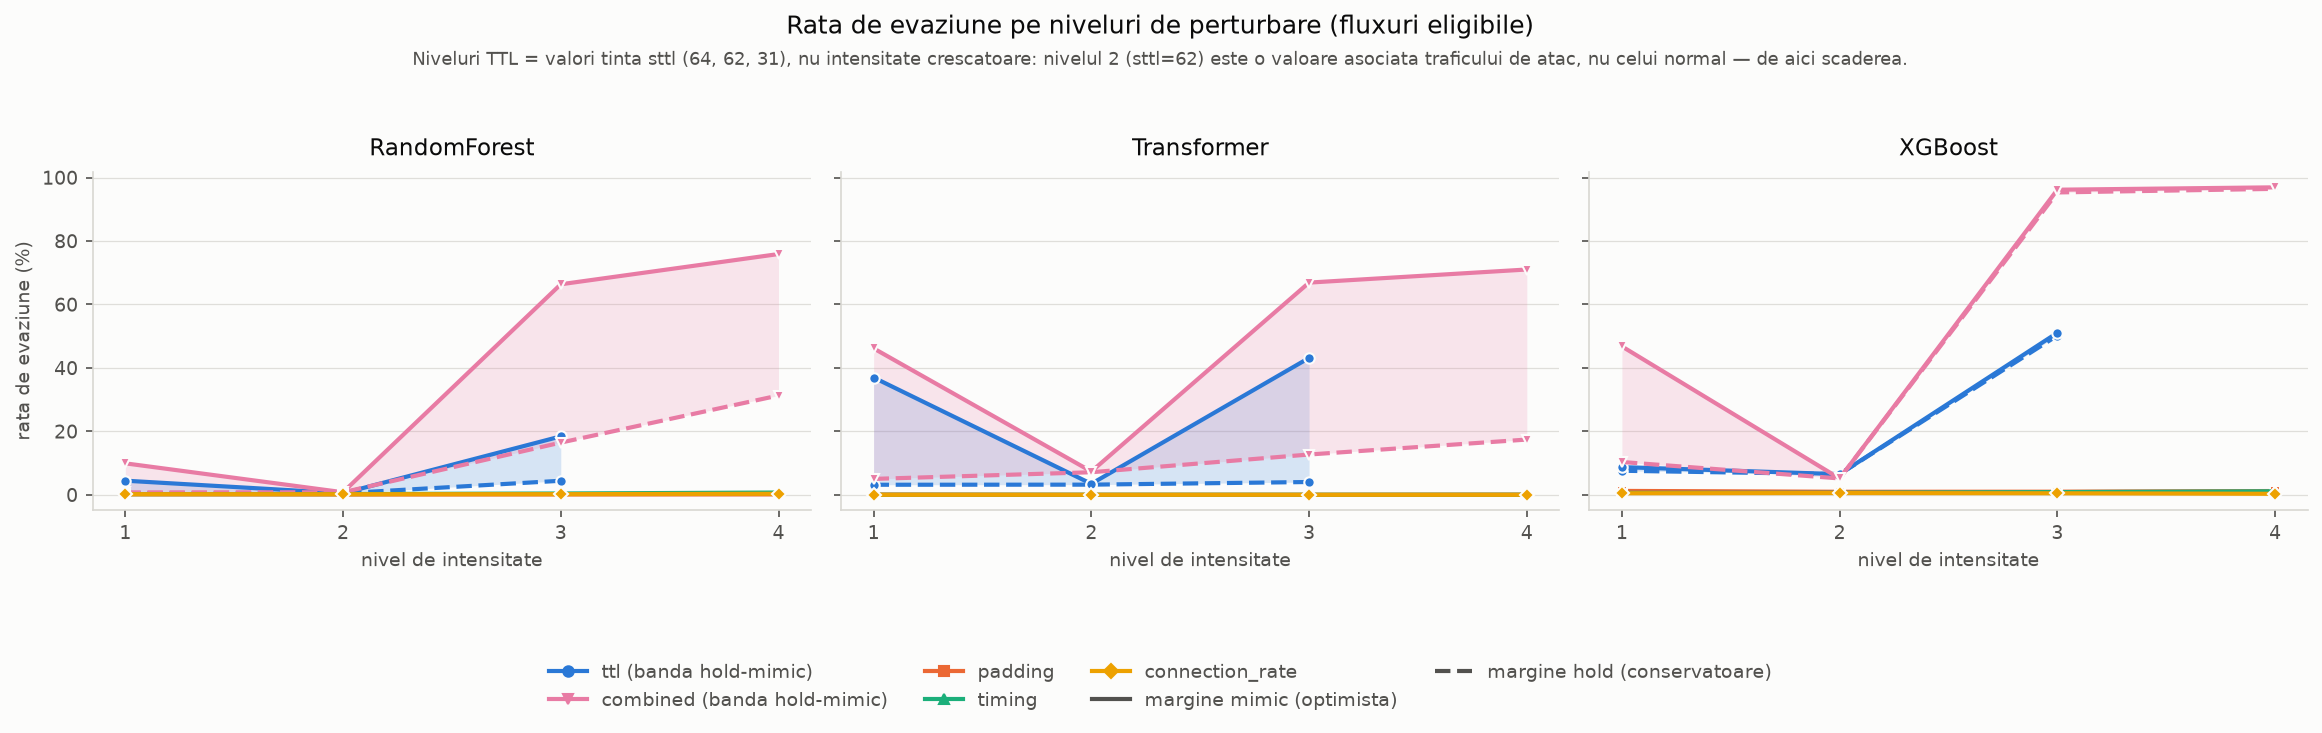
\includegraphics[width=0.95\textwidth]{figs/evasion_curves.png}
    \caption{Rata de evaziune în funcție de tipul transformării și de nivelul de intensitate}
    \label{fig:curbe}
\end{figure}

Costul practic al acestei perturbări pentru un atacator este esențial pentru interpretarea rezultatului. Modificarea valorii TTL a pachetelor emise se realizează printr-un singur apel de configurare a socketului și nu necesită nicio cunoaștere a sistemului de detecție. Valorile-țintă folosite se află peste limita inferioară discutată în subsecțiunea~\ref{subsec:admisibile}, deci rămân compatibile cu păstrarea funcționalității atacului în modelul de amenințare adoptat. Este, prin urmare, o perturbare cu cost practic nul.

\subsection{Explicația: valoarea TTL este un artefact al capturii}\label{subsec:artefact}

Analiza distribuției valorii TTL explică rezultatul. În partiția de antrenare, valoarea dominantă a traficului legitim este 31, prezentă în $70{,}5\%$ dintre fluxuri, în timp ce în fiecare clasă de atac valoarea dominantă este 254, cu ponderi care merg de la $59{,}5\%$ pe \textit{Exploits} până la $100\%$ pe \textit{Shellcode}. Această separare face ca TTL-ul sursă să fie, dintre toate cele 42 de caracteristici, cea mai corelată cu eticheta, cu un coeficient de $0{,}69$.

Separarea nu descrie însă o proprietate a atacurilor, ci una a mediului de captură: generatorul de trafic malițios s-a aflat la o distanță fixă, în număr de salturi, față de senzorul care a înregistrat traficul. Că este vorba despre o corelație și nu despre o regulă rezultă din faptul că traficul legitim conține el însuși peste 11\,000 de fluxuri cu valoarea 254, adică aproximativ o cincime din traficul legitim al partiției de antrenare.

Modelele au învățat, prin urmare, o particularitate a procesului de generare a datelor, pe care o folosesc ca principal criteriu de decizie. Perturbarea nu exploatează o slăbiciune a arhitecturii, ci una a setului de date, observație cu implicații care depășesc modelele evaluate aici.

\subsection{Nivelurile de intensitate nu formează o scară monotonă}\label{subsec:nemonoton}

Rezultatele din figura~\ref{fig:curbe} prezintă o scădere aparent anormală la nivelul intermediar al transformării TTL: pentru Transformer, rata scade de la $36{,}98\%$ la nivelul 1 la $3{,}47\%$ la nivelul 2, revenind la $43{,}15\%$ la nivelul 3.

Comportamentul nu este o eroare, ci consecința directă a modului în care sunt definite nivelurile. Ele reprezintă \emph{valori-țintă} distincte, nu intensități crescătoare ale aceleiași modificări. Valoarea corespunzătoare nivelului 2 este o valoare frecvent asociată traficului malițios în acest set, astfel încât adoptarea ei nu apropie fluxul de profilul traficului legitim.

Explicația a fost verificată prin măsurarea directă a proporției de fluxuri care ajung, sub politica optimistă, la valoarea contorului de context caracteristică traficului normal: proporția este de 100\% la nivelul 1, \textbf{0\%} la nivelul 2 și 100\% la nivelul 3. Nivelul intermediar nu produce semnătura traficului legitim, deci nu are motive să producă evaziune.

\subsection{Lățimea intervalelor}\label{subsec:latime}

Intervalele din tabelul~\ref{tab:evaziune} au lățimi foarte diferite, iar această variație este informativă. Pentru XGBoost, intervalul transformării TTL are o lățime sub o unitate procentuală ($50{,}2$ -- $51{,}1$), ceea ce arată că rezultatul nu depinde practic de ipoteza adoptată privind contorul de context. Pentru Transformer, același interval se întinde de la $4{,}0$ la $43{,}2$, deci aproape zece ori mai larg.

Interpretarea este directă: în primul caz, decizia modelului se schimbă din cauza valorii TTL însăși. În al doilea caz, o parte substanțială a efectului depinde de faptul că perturbarea reușește sau nu să reproducă și semnătura de context asociată. Raportarea unei valori unice ar fi ascuns tocmai această distincție, care este relevantă pentru evaluarea realismului atacului.

\subsection{Compoziția rezultatelor}\label{subsec:compozitie}

Tabelul~\ref{tab:compozitie} prezintă distribuția celor trei rezultate definite în subsecțiunea~\ref{subsec:rezultate} pentru transformarea TTL la intensitate maximă, sub politica optimistă.

\begin{table}[!ht]
    \caption{Compoziția rezultatelor pentru transformarea TTL la intensitate maximă (\%)}
    \centering
    \begin{tabular}{|l|c|c|c|}
        \hline
        \textbf{Model} & \textbf{Corect} & \textbf{Alt atac} & \textbf{Evaziune} \\
        \hline
        Random Forest & 65,56 & 16,02 & 18,42 \\
        \hline
        XGBoost & 40,71 & 8,22 & \textbf{51,07} \\
        \hline
        Transformer & 13,19 & \textbf{43,66} & 43,15 \\
        \hline
    \end{tabular}
    \label{tab:compozitie}
\end{table}

Cele trei modele reacționează calitativ diferit la aceeași perturbare. Random Forest păstrează clasificarea corectă pentru majoritatea fluxurilor. Modelul cu XGBoost trece direct la clasa traficului legitim. Transformer pierde aproape complet clasificarea corectă (sub 14\%) dar redistribuie fluxurile aproape în mod egal între evaziune și confuzie cu alte categorii de atac. Din perspectiva unui sistem de detecție operațional, ultimele două comportamente sunt foarte diferite: în cazul confuziei, alarma se declanșează în continuare.

Aceeași defalcare, extinsă la toate variantele și la toate cele trei modele, este prezentată în figura~\ref{fig:outcomes}. Citită pe verticală, ea arată că diferența dintre modele nu ține de o singură transformare, ci se păstrează pe întreaga grilă.

\begin{figure}[H]
    \centering
    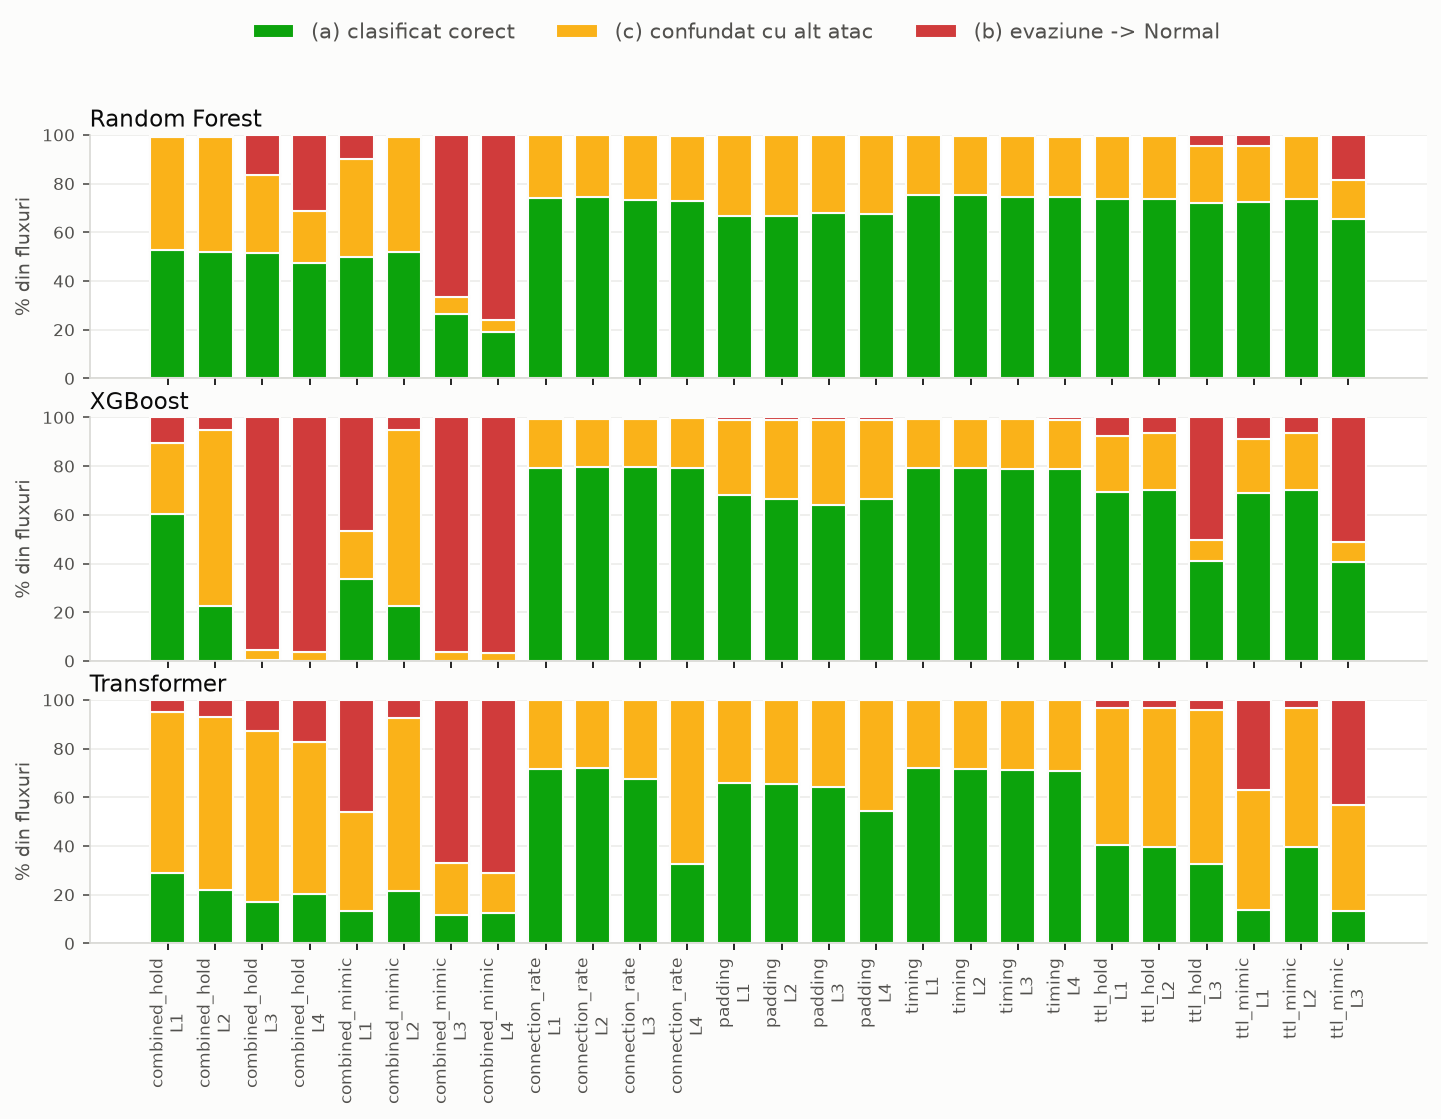
\includegraphics[width=\textwidth]{figs/evasion_outcomes_toate.png}
    \caption{Compoziția rezultatelor pe cele 26 de variante realizabile, pentru cele trei modele. Roșul apare masiv doar la variantele care ating valoarea TTL, în timp ce umplutura, temporizarea și reducerea contoarelor lasă compoziția aproape neschimbată la toate trei. Diferența dintre modele se citește pe verticală, la aceeași poziție pe axă.}
    \label{fig:outcomes}
\end{figure}

\subsection{Modificarea probabilităților de clasificare}\label{subsec:incredere}

Dincolo de eticheta finală, perturbarea modifică distribuția de probabilitate produsă de model. Tabelul~\ref{tab:incredere} prezintă valorile medii înainte și după transformarea TTL la intensitate maximă.

\begin{table}[!ht]
    \caption{Deplasarea probabilităților medii sub transformarea TTL la intensitate maximă}
    \centering
    \begin{tabular}{|l|c|c|}
        \hline
        \textbf{Model} & \textbf{$P(\textit{Normal})$} & \textbf{$P(\text{clasa reală})$} \\
        \hline
        Random Forest & 0,027 $\rightarrow$ 0,248 & 0,684 $\rightarrow$ 0,455 \\
        \hline
        XGBoost & 0,022 $\rightarrow$ 0,525 & 0,750 $\rightarrow$ 0,394 \\
        \hline
        Transformer & 0,013 $\rightarrow$ 0,419 & 0,694 $\rightarrow$ \textbf{0,148} \\
        \hline
    \end{tabular}
    \label{tab:incredere}
\end{table}

În urma perturbării, toate cele trei modele atribuie, în medie, o probabilitate mai redusă clasei reale și o probabilitate mai mare clasei normale. Cea mai mare scădere a probabilității asociate clasei reale apare în cazul Transformerului, de la 0,694 la 0,148. Pentru XGBoost, probabilitatea medie atribuită clasei normale ajunge la 0,525, depășind valoarea corespunzătoare clasei reale. Rezultatele arată că transformarea TTL afectează nu numai etichetele prezise, ci și distribuția probabilităților între clase.
\subsection{Defalcarea pe clase de atac}\label{subsec:perclasa-evaziune}

Rata globală ascunde diferențe importante între categoriile de atac. Tabelul~\ref{tab:evaziune-clase} prezintă defalcarea pentru transformarea TTL la intensitate maximă, sub politica optimistă.

\begin{table}[!ht]
    \caption{Rata de evaziune pe clase de atac, transformare TTL la intensitate maximă (\%)}
    \centering
    \begin{tabular}{|l|c|c|c|}
        \hline
        \textbf{Clasă} & \textbf{RF} & \textbf{XGB} & \textbf{Transformer} \\
        \hline
        Shellcode & 24,9 & \textbf{100,0} & 25,7 \\
        \hline
        Worms & 13,6 & \textbf{100,0} & 18,2 \\
        \hline
        Reconnaissance & 4,8 & \textbf{95,9} & 10,3 \\
        \hline
        Fuzzers & 67,7 & 89,8 & 49,8 \\
        \hline
        Exploits & 17,1 & 87,5 & 16,1 \\
        \hline
        Backdoor & 72,4 & 66,4 & 38,4 \\
        \hline
        DoS & 24,5 & 66,5 & 25,0 \\
        \hline
        Analysis & 66,1 & 63,8 & 41,4 \\
        \hline
        Generic & \textbf{1,5} & \textbf{5,5} & \textbf{67,6} \\
        \hline
    \end{tabular}
    \label{tab:evaziune-clase}
\end{table}

Se pot face trei observații.

Pentru XGBoost, toate fluxurile din clasele \textit{Shellcode} și \textit{Worms} incluse în evaluare sunt reclasificate drept trafic normal. Cele două clase sunt reprezentate prin 378, respectiv 44 de observații în partiția de testare, astfel încât valorile obținute sunt analizate în raport cu dimensiunea redusă a eșantioanelor. Această limitare este semnalată și în fișierele de rezultate. Rezultatele sugerează o vulnerabilitate mai mare a claselor slab reprezentate, însă nu sunt suficiente pentru a stabili o relație generală între frecvența unei clase și rata sa de evaziune.
A doua: clasa \textit{Generic}, cea mai bine clasificată de toate modelele conform tabelului~\ref{tab:perclasa}, rezistă aproape complet la ansamblurile de arbori, $1{,}5\%$ și $5{,}5\%$, dar cedează masiv la Transformer, cu $67{,}6\%$. Este singura clasă la care ordinea modelelor se inversează complet.

A treia: nu există o corelație simplă între calitatea clasificării inițiale și rezistența la perturbare. Clasa \textit{Analysis}, practic neclasificabilă pe trafic nemodificat, prezintă rate de evaziune comparabile cu ale unor clase bine clasificate. Rezistența la perturbare este, prin urmare, o proprietate distinctă de acuratețe, nu o consecință a ei, concluzie consistentă cu cea formulată la nivel global.

Defalcarea completă pe clase și niveluri pentru Transformer este prezentată în figura~\ref{fig:perclasa-tr}.

\begin{figure}[H]
    \centering
    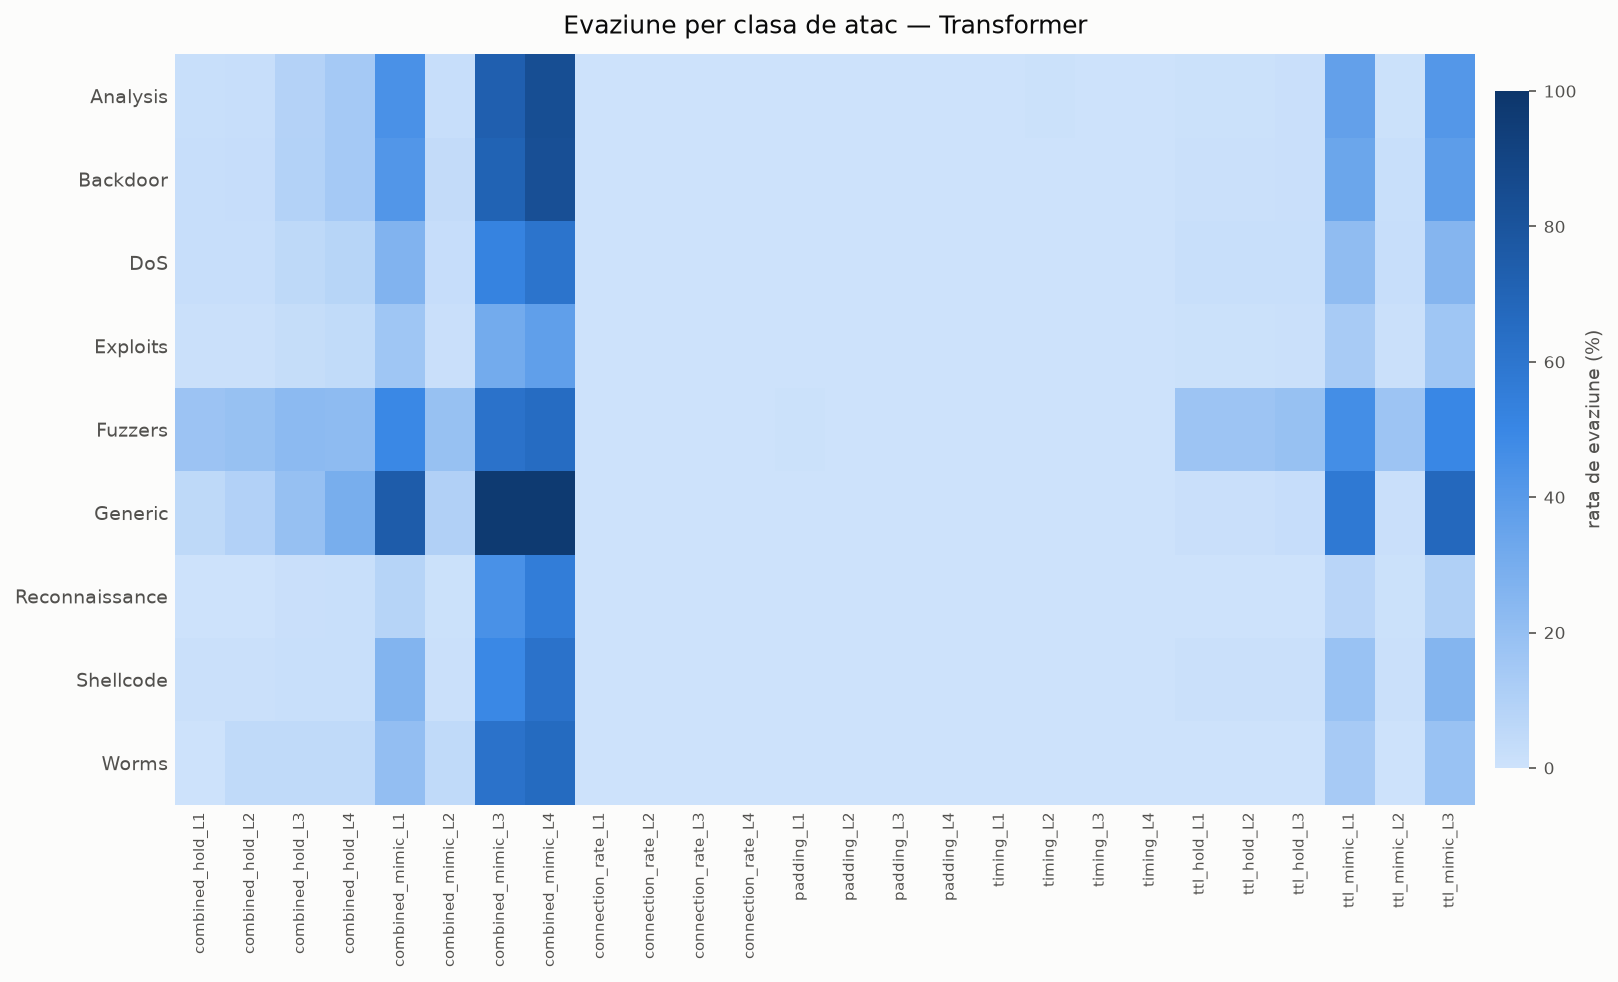
\includegraphics[width=0.92\textwidth]{figs/evasion_per_class_transformer.png}
    \caption{Rata de evaziune pe clase de atac și niveluri, pentru Transformer}
    \label{fig:perclasa-tr}
\end{figure}

\subsection{Intensitatea minimă necesară}\label{subsec:intensitate}

O rată de evaziune ridicată obținută abia la intensitatea maximă are o semnificație practică diferită de una obținută încă de la prima treaptă. Tabelul~\ref{tab:intensitate} prezintă, pentru transformarea TTL sub politica optimistă, proporția fluxurilor care evadează la un moment dat și nivelul median la care se produce prima evaziune.

\begin{table}[!ht]
    \caption{Intensitatea minimă la care se produce evaziunea (transformare TTL)}
    \centering
    \begin{tabular}{|l|c|c|r|}
        \hline
        \textbf{Model} & \textbf{Evadează} & \textbf{Nivel median} & \textbf{La nivelul 1} \\
        \hline
        Random Forest & 18,4\% & 3,0 & 2\,011 \\
        \hline
        XGBoost & 51,1\% & 3,0 & 3\,868 \\
        \hline
        Transformer & 43,2\% & \textbf{1,0} & \textbf{16\,752} \\
        \hline
    \end{tabular}
    \label{tab:intensitate}
\end{table}

Ansamblurile de arbori cedează majoritar abia la nivelul cel mai intens. Transformer are nivelul median egal cu 1: pentru aceasta, peste 16\,000 de fluxuri evadează încă de la prima treaptă de perturbare, deci nu este necesară deplasarea completă către profilul traficului legitim.

\section{Analiza de sensibilitate}\label{sec:rezultate-o4}

\subsection{Profilurile de importanță}\label{subsec:profiluri}

Tabelul~\ref{tab:importanta} prezintă primele trei caracteristici după importanța determinată prin permutare, împreună cu ponderea caracteristicii dominante în capacitatea totală de detecție.

\begin{table}[H]
    \caption{Caracteristicile cele mai importante și concentrarea capacității de detecție}
    \centering
    \begin{tabular}{|l|l|l|l|c|}
        \hline
        \textbf{Model} & \textbf{1} & \textbf{2} & \textbf{3} & \textbf{Pondere dom.} \\
        \hline
        Random Forest & TTL sursă & protocol & fereastră & 19,8\% \\
        \hline
        XGBoost & \textbf{TTL sursă} & dim. medie dest. & debit dest. & \textbf{54,6\%} \\
        \hline
        Transformer & \textbf{TTL destinație} & TTL sursă & protocol & \textbf{57,0\%} \\
        \hline
    \end{tabular}
    \label{tab:importanta}
\end{table}

Profilurile explică integral rezultatele din secțiunea~\ref{sec:rezultate-o3}. Modelul cu XGBoost concentrează $54{,}6\%$ din capacitatea sa de detecție într-o singură caracteristică, pe care atacatorul o modifică fără cost: de aici rata de evaziune de peste $50\%$. Random Forest distribuie aceeași caracteristică pe doar $19{,}8\%$, iar rata sa de evaziune este corespunzător mai mică. Comportamentul este consistent cu predicția teoretică din subsecțiunea~\ref{subsec:arbori}: selecția aleatoare a caracteristicilor la construirea nodurilor împiedică concentrarea deciziei.

Transformer prezintă profilul cel mai interesant: caracteristica sa dominantă este valoarea TTL a pachetelor \emph{de răspuns}, deci una generată de victimă și inaccesibilă atacatorului. Comparația vizuală a celor trei profiluri este prezentată în figura~\ref{fig:importanta}.

\begin{figure}[!ht]
    \centering
    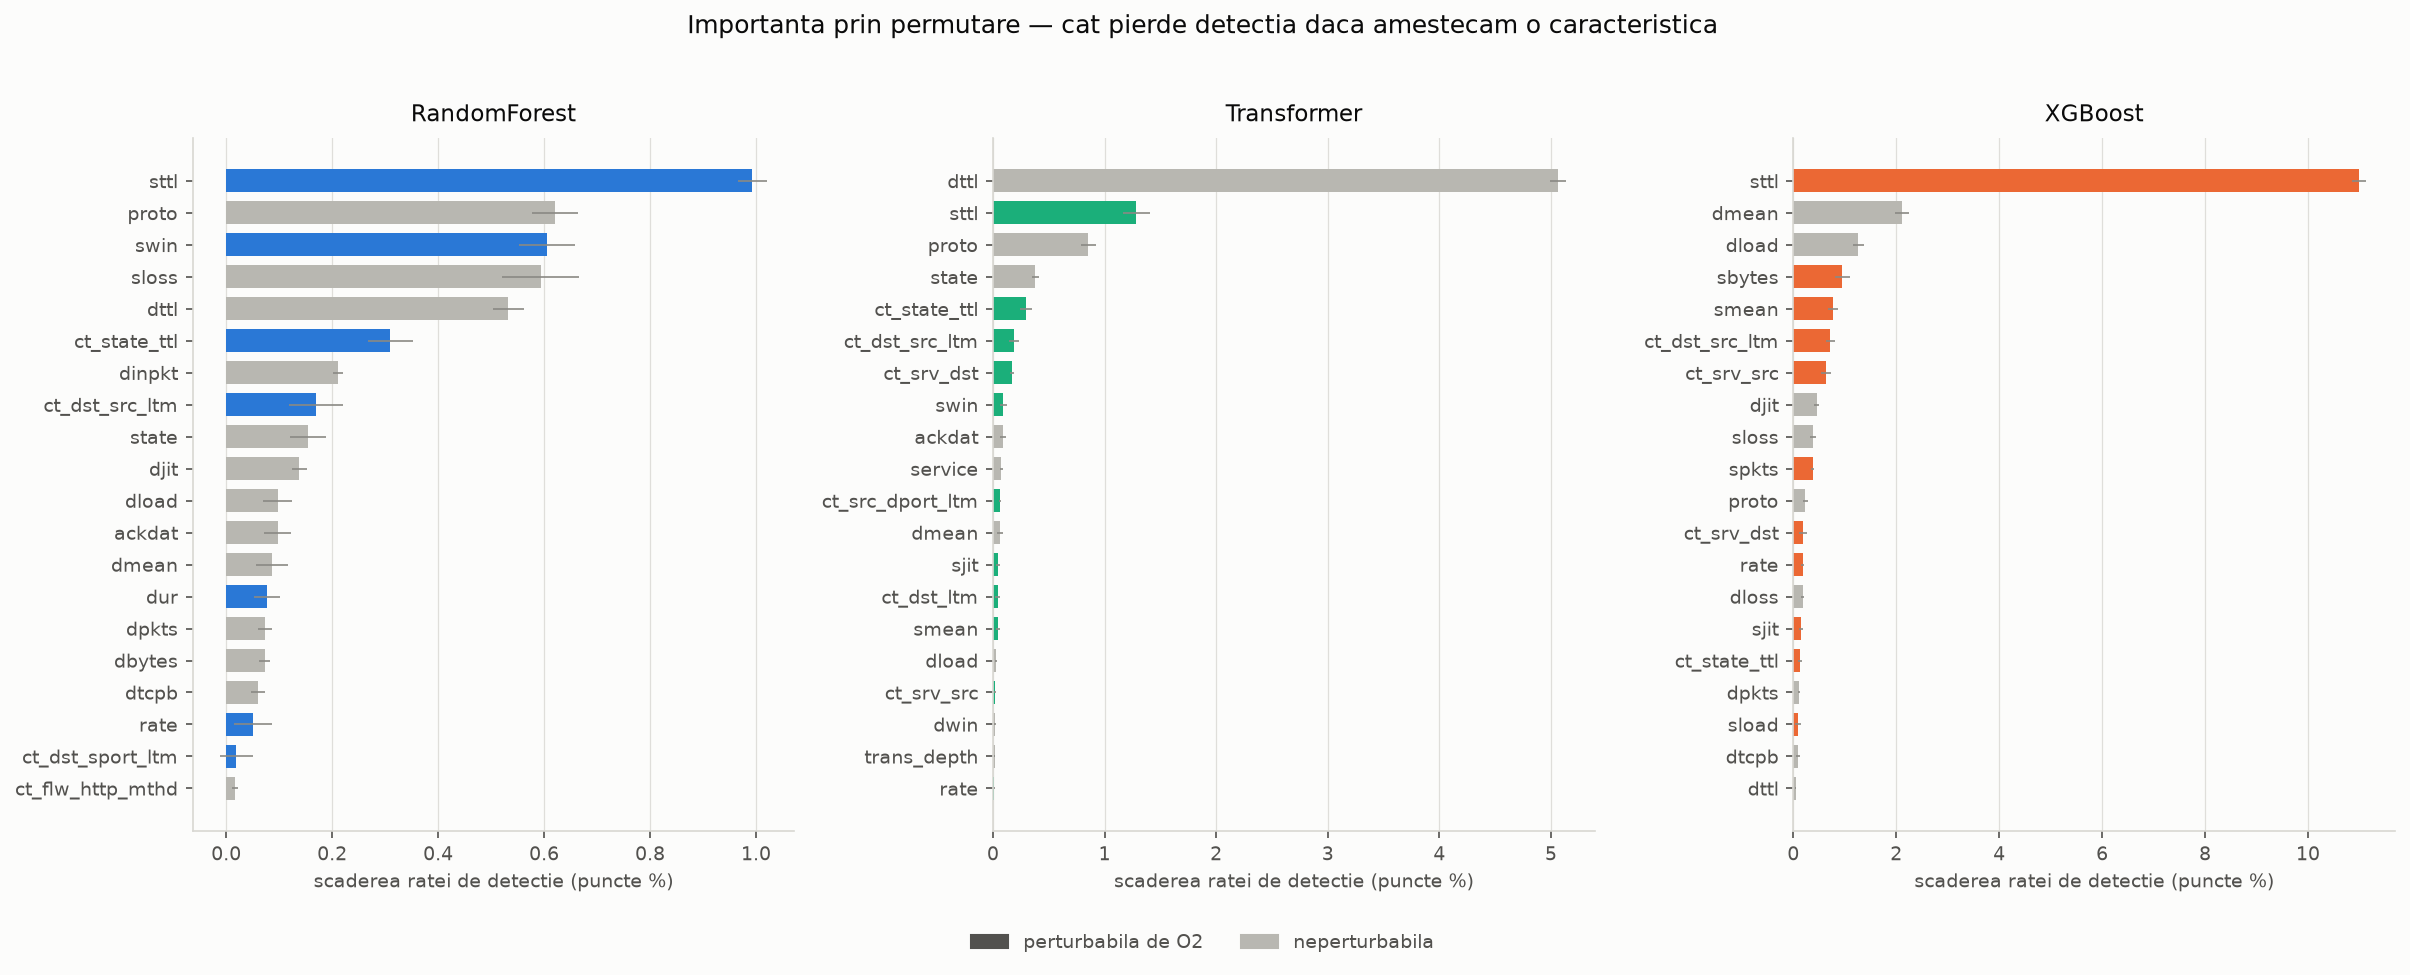
\includegraphics[width=0.95\textwidth]{figs/sensitivity_importance.png}
    \caption{Importanța prin permutare a caracteristicilor, pentru cele trei modele}
    \label{fig:importanta}
\end{figure}

\subsection{Fracțiunea accesibilă atacatorului}\label{subsec:fractiune}

Aplicând definiția fracțiunii accesibile din subsecțiunea~\ref{subsec:accesibila} se obțin valorile din tabelul~\ref{tab:accesibila}.

\begin{table}[!ht]
    \caption{Fracțiunea din capacitatea de detecție aflată la îndemâna atacatorului}
    \centering
    \begin{tabular}{|l|c|c|}
        \hline
        \textbf{Model} & \textbf{Pierdere totală} & \textbf{Fracțiune accesibilă $\rho$} \\
        \hline
        Random Forest & 5,02 & 53,6\% \\
        \hline
        XGBoost & 20,15 & \textbf{84,1\%} \\
        \hline
        Transformer & 8,89 & \textbf{26,0\%} \\
        \hline
    \end{tabular}
    \label{tab:accesibila}
\end{table}

Valorile ordonează modelele exact invers față de rezistența lor observată. Modelul cu XGBoost are $84{,}1\%$ din capacitatea de detecție în caracteristici modificabile și cedează cel mai mult. Transformer are doar $26{,}0\%$ și cedează cel mai puțin la transformările realizabile.

Aceasta este constatarea centrală a lucrării. Rezistența superioară a modelului Transformer \textbf{nu provine dintr-o reprezentare mai bună}, ci din faptul că modelul se sprijină preponderent pe informație pe care atacatorul nu o poate atinge. Distincția formulată teoretic în subsecțiunea~\ref{subsec:comparatie} este astfel tranșată empiric, în favoarea celei de-a doua explicații.

Confirmarea directă vine din varianta de referință cu constrângeri relaxate, singura care modifică și caracteristica generată de victimă. Sub această variantă, rata de evaziune a rețelei urcă la $71{,}1\%$, față de $43{,}2\%$ la transformarea realizabilă echivalentă. Prin contrast, pentru XGBoost valoarea rămâne neschimbată la $51{,}1\%$, deoarece acesta nu se sprijină semnificativ pe caracteristica respectivă. Se reamintește că această variantă nu descrie un atac practic și nu poate fi raportată alături de rezultatele realizabile, întrucât rolul ei este strict diagnostic.

\subsection{Confirmarea prin scenariul cu constrângeri relaxate}\label{subsec:relaxat}

Varianta de referință care modifică suplimentar caracteristica generată de victimă oferă o confirmare directă a interpretării. Rezultatele sunt prezentate în tabelul~\ref{tab:relaxat}.

\begin{table}[!ht]
    \caption{Comparație între transformarea realizabilă și scenariul cu constrângeri relaxate}
    \centering
    \begin{tabular}{|l|c|c|c|}
        \hline
        \textbf{Model} & \textbf{Realizabil} & \textbf{Relaxat} & \textbf{Diferență} \\
        \hline
        Random Forest & 18,4\% & 33,0\% & $+14{,}6$ \\
        \hline
        XGBoost & 51,1\% & 51,1\% & \textbf{$0{,}0$} \\
        \hline
        Transformer & 43,2\% & \textbf{71,1\%} & \textbf{$+27{,}9$} \\
        \hline
    \end{tabular}
    \label{tab:relaxat}
\end{table}

Diferențele reproduc exact ordinea prezisă de fracțiunile accesibile din tabelul~\ref{tab:accesibila}. Pentru XGBoost, relaxarea constrângerii nu schimbă absolut nimic: acesta nu folosește caracteristica generată de victimă, deci accesul suplimentar la ea nu aduce niciun avantaj atacatorului. Pentru Transformer, aceeași relaxare adaugă aproape 28 de puncte procentuale.

Valoarea scenariului relaxat este strict diagnostică: el separă întrebarea „cât de mult se sprijină modelul pe această informație” de întrebarea „cât poate obține un atacator real”.

\subsection{Corelația dintre importanță și evaziune}\label{subsec:corelatie}

Obiectivul formulat în capitolul~\ref{ch:obiective} cere punerea în corespondență a ratei de evaziune cu importanța caracteristicilor afectate. Tabelul~\ref{tab:corelatie} prezintă coeficienții de corelație a rangurilor, calculați pe cele 26 de variante realizabile.

\begin{table}[!ht]
    \caption{Corelația dintre masa de importanță afectată și rata de evaziune}
    \centering
    \begin{tabular}{|l|c|c|c|}
        \hline
        \textbf{Model} & \textbf{$\rho$ Spearman} & \textbf{$p$} & \textbf{$n$} \\
        \hline
        Random Forest & \textbf{0,954} & $<0{,}0001$ & 26 \\
        \hline
        XGBoost & 0,882 & $<0{,}0001$ & 26 \\
        \hline
        Transformer & 0,830 & $<0{,}0001$ & 26 \\
        \hline
    \end{tabular}
    \label{tab:corelatie}
\end{table}

Corelațiile sunt puternice și semnificative pentru toate cele trei modele: transformările care afectează o masă mai mare de importanță produc o evaziune mai mare. Relația este ilustrată în figura~\ref{fig:corelatie}.

\begin{figure}[!ht]
    \centering
    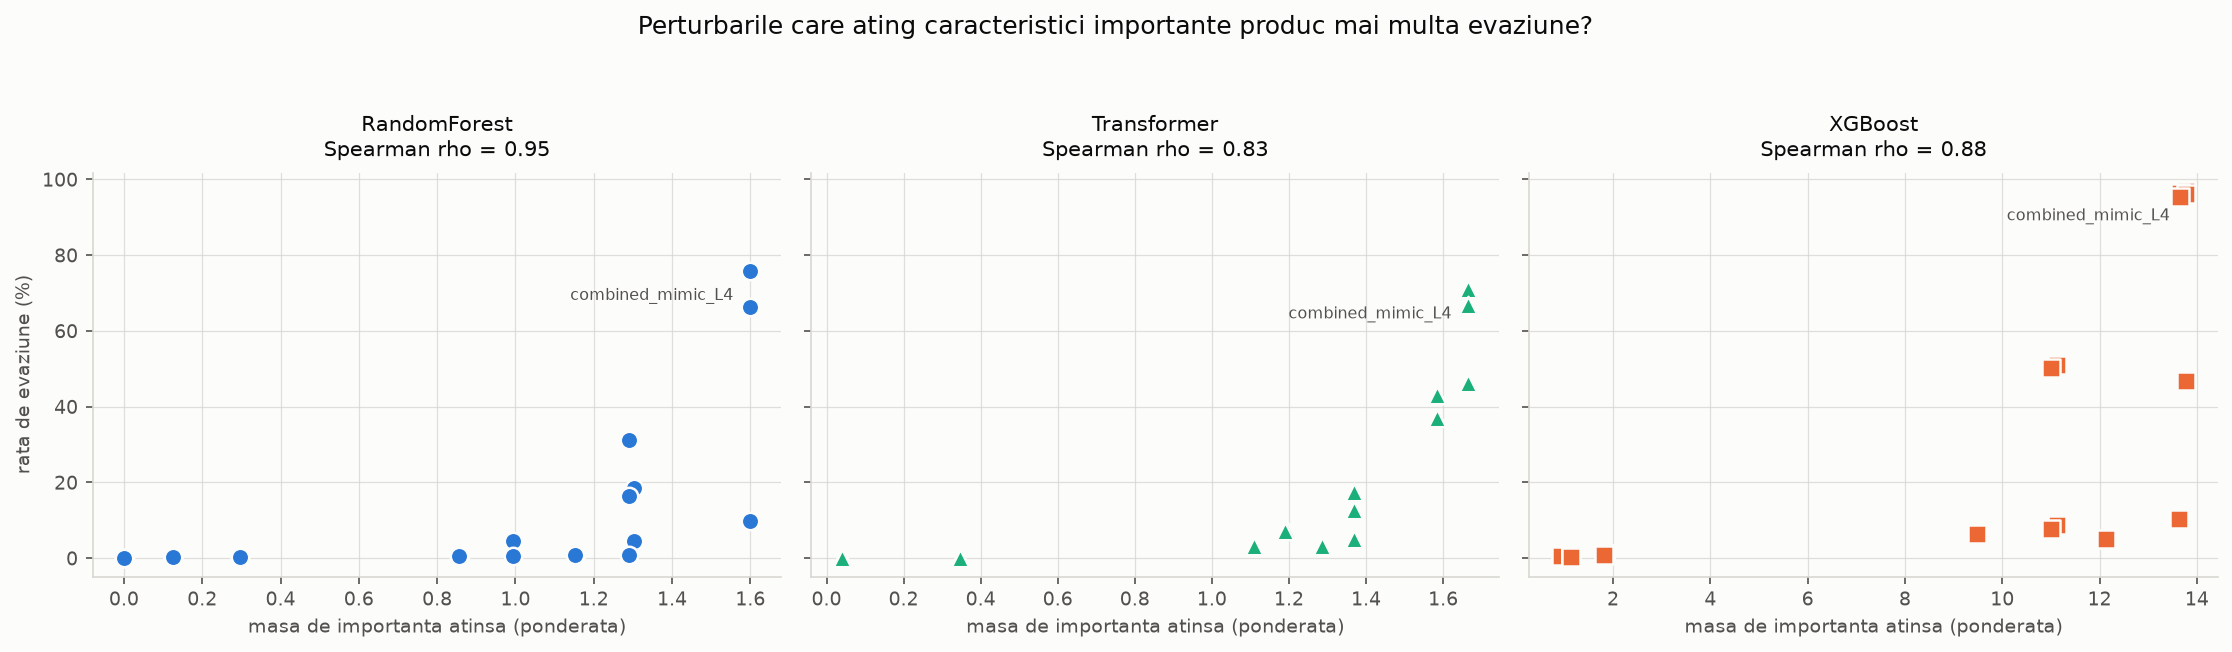
\includegraphics[width=0.88\textwidth]{figs/sensitivity_importance_vs_evasion.png}
    \caption{Relația dintre masa de importanță afectată și rata de evaziune}
    \label{fig:corelatie}
\end{figure}

Rezultatul validează metodologia: importanța determinată prin permutare, calculată independent de experimentul de evaziune, prezice ce transformări vor fi eficiente. Alegerea metricii comensurabile din subsecțiunea~\ref{subsec:comensurabil} este cea care face posibilă această comparație directă.

\subsection{Clasele atractor}\label{subsec:atractor}

Analiza rezultatului de tip (c) arată că fluxurile care rămân semnalate nu se distribuie uniform între clasele de atac, ci converg către o clasă preferată, diferită pentru fiecare model. Pentru XGBoost, între $67{,}6\%$ și $95{,}8\%$ dintre fluxurile provenite din orice clasă sursă ajung la clasa \textit{Analysis}. Pentru Random Forest, clasa preferată este \textit{Backdoor}, iar pentru Transformer, \textit{DoS}.

Fenomenul nu este întâmplător. Clasele \textit{Analysis} și \textit{Backdoor} sunt exact cele cu cele mai slabe scoruri $F1$ din tabelul~\ref{tab:perclasa}, cu valori între $0{,}003$ și $0{,}116$. Clasa atractor este regiunea din spațiul caracteristicilor în care modelul nu are un angajament ferm: atunci când perturbarea îndepărtează fluxul de clasa sa, acesta este împins către zona de incertitudine maximă. Distribuția destinațiilor este prezentată în figura~\ref{fig:destinatii}.

\begin{figure}[H]
    \centering
    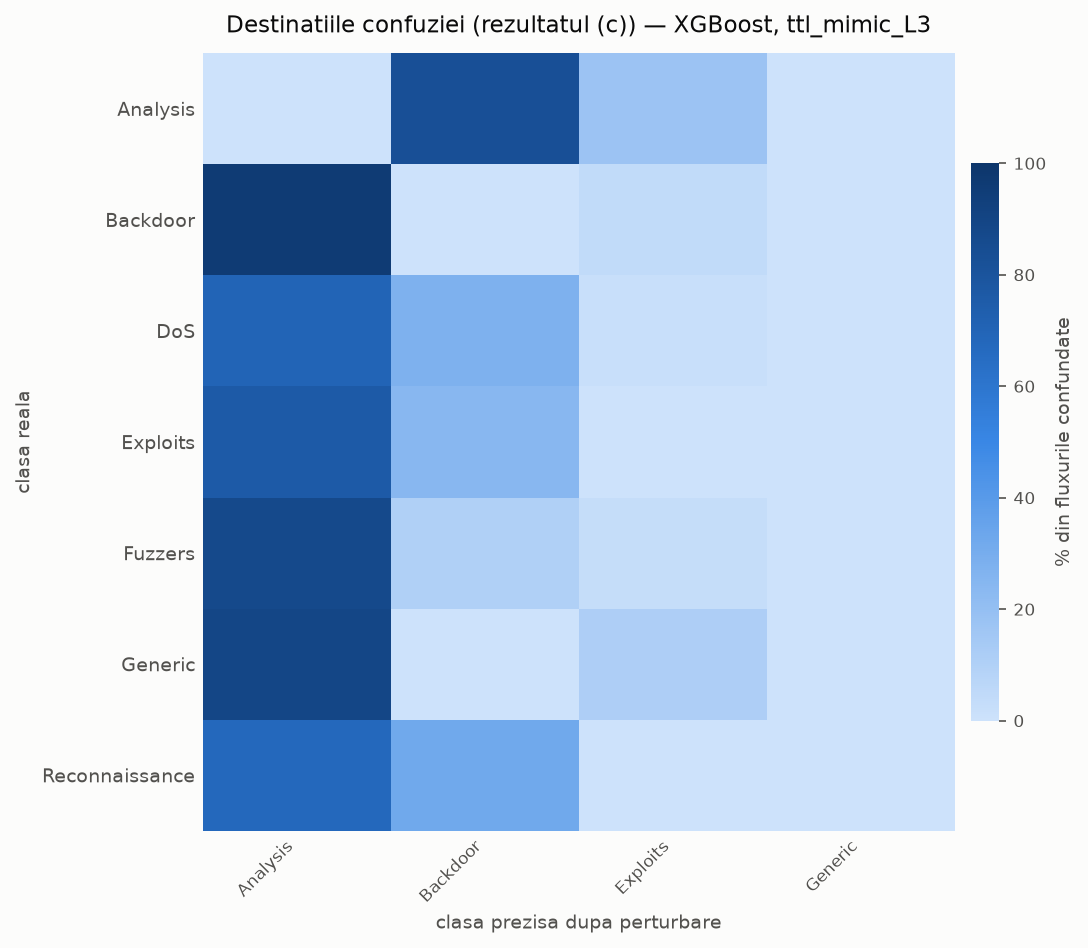
\includegraphics[width=0.88\textwidth]{figs/sensitivity_destinations_xgboost.png}
    \caption{Distribuția claselor de destinație pentru fluxurile perturbate care rămân semnalate}
    \label{fig:destinatii}
\end{figure}

\subsection{Proximitatea față de granița de decizie}\label{subsec:proximitate}

Se pune întrebarea dacă fluxurile care evadează erau deja incerte înainte de perturbare. Tabelul~\ref{tab:proximitate} compară probabilitatea medie atribuită clasei reale, pe traficul nemodificat, pentru fluxurile care ulterior evadează față de cele care nu evadează.

\begin{table}[!ht]
    \caption{Încrederea inițială a modelului, pentru fluxurile care evadează și pentru celelalte}
    \centering
    \begin{tabular}{|l|c|c|c|}
        \hline
        \textbf{Model} & \textbf{Evadate} & \textbf{Ne-evadate} & \textbf{Diferență} \\
        \hline
        Random Forest & 0,359 & 0,757 & \textbf{$+0{,}398$} \\
        \hline
        XGBoost & 0,653 & 0,850 & $+0{,}197$ \\
        \hline
        Transformer & 0,806 & 0,609 & \textbf{$-0{,}197$} \\
        \hline
    \end{tabular}
    \label{tab:proximitate}
\end{table}

Pentru ansamblurile de arbori, diferența este pozitivă și substanțială: evaziunea se concentrează pe fluxurile față de care modelul era deja nesigur, ceea ce corespunde intuiției. Pentru Transformer, diferența este \textbf{negativă}: modelul cedează tocmai pe fluxurile de care era \emph{mai} sigur.

Rezultatul este contraintuitiv și are o implicație practică importantă: încrederea ridicată a acestui model nu constituie un indicator de robustețe. Un mecanism de apărare care ar trata predicțiile de încredere mare drept fiabile ar fi ineficient exact acolo unde este mai necesar.

\subsection{Limita atribuirii pe o singură caracteristică}\label{subsec:limitaatrib}

Analiza res\-trân\-să la clasa \textit{Generic} ilus\-trea\-ză li\-mi\-ta\-rea an\-ti\-ci\-pa\-tă te\-o\-re\-tic în subsecțiunea~\ref{subsec:limita}. Pentru Transformer, importanța se distribuie pe această clasă între trei caracteristici cu ponderi apropiate, $33{,}8\%$, $32{,}9\%$ și $23{,}1\%$, niciuna dintre ele nefiind, luată separat, suficientă pentru a explica prăbușirea detecției observată sub perturbare.

Constatarea confirmă că importanța atribuită individual constituie o limită inferioară a vulnerabilității, nu o estimare a ei, și justifică retroactiv decizia centrală de proiectare din capitolul~\ref{ch:analysis}: propagarea consistentă a dependențelor. O metodologie care ar fi perturbat caracteristicile izolat, fără propagare, nu ar fi produs substituția coerentă necesară și ar fi subestimat sistematic vulnerabilitatea măsurată.

Această etapă a necesitat și o corecție de implementare, descrisă în secțiunea~\ref{sec:implsensibilitate}: pe o singură clasă, permutarea internă a valorilor nu rupe legătura cu eticheta atunci când caracteristica este cvasiconstantă în interiorul clasei, iar importanța apare fals ca nulă. Substituția dintr-o distribuție donoare externă a corectat măsurătoarea.

\section{Efectul antrenării adversariale}\label{sec:rezultate-o6}

Secțiunea prezintă rezultatele obținute prin reantrenarea celor trei clasificatoare pe seturi care conțin variante perturbate, conform construcției din secțiunea~\ref{sec:antrenare}. Verificările de integritate ale montajului au fost prezentate separat în subsecțiunea~\ref{subsec:val-adversarial} și au precedat citirea oricărui rezultat.

\subsection{Configurația experimentului}\label{subsec:o6-config}

Au fost antrenate treizeci de modele: trei grupuri, trei repetări cu \textit{seed}-uri distincte și trei familii de clasificatoare, la care se adaugă un al patrulea grup, cu o singură repetare, destinat testului de generalizare din subsecțiunea~\ref{subsec:o6-generalizare}. Compoziția seturilor este cea din subsecțiunea~\ref{subsec:val-adversarial}: 294\,682 de rânduri pentru ambele grupuri augmentate, identice ca dimensiune și distribuție a claselor.

Antrenarea a durat 89 de minute pentru ansamblurile de arbori și 282 de minute pentru Transformer, cele două putând rula simultan întrucât folosesc resurse diferite. Evaluarea celor treizeci de modele a durat 26 de minute.

Un rezultat colateral al antrenării merită consemnat, pentru că privește stabilitatea măsurătorilor care urmează. Numărul de epoci până la cel mai bun scor de validare a variat, la cele zece rulări ale rețelei, între 10 și 48, deși în interiorul unui grup singura diferență între rulări este \textit{seed}-ul. Amplitudinea confirmă necesitatea repetării: un grup de control evaluat cu un singur \textit{seed} ar fi putut proveni din oricare dintre cele două extreme.

\subsection{Mulțimea comună de măsurare}\label{subsec:o6-cohorta}

Ratele de evaziune se raportează la intersecția fluxurilor semnalate pe trafic nemodificat de toate rulările aceleiași familii, conform subsecțiunii~\ref{subsec:cohorta}. Dimensiunile obținute sunt prezentate în tabelul~\ref{tab:o6-cohorte}.

\begin{table}[!ht]
    \caption{Mulțimea comună per familie de modele}
    \centering
    \begin{tabular}{|l|c|c|c|}
        \hline
        \textbf{Model} & \textbf{Eligibile per rulare} & \textbf{Mulțimea comună} & \textbf{Din fluxurile de atac} \\
        \hline
        Random Forest & 45\,106--45\,250 & 45\,001 & 99,27\,\% \\
        \hline
        XGBoost & 44\,237--44\,658 & 43\,637 & 96,26\,\% \\
        \hline
        Transformer & 45\,173--45\,307 & 44\,982 & 99,23\,\% \\
        \hline
    \end{tabular}
    \label{tab:o6-cohorte}
\end{table}

Intersecția a costat între 0,7\,\% și 3,7\,\% din fluxurile de atac, deci comparațiile se fac practic pe întreaga populație, nu pe un rest îngust. Această mulțime a fost construită împotriva unei situații anume, aceea în care un model pare robust doar pentru că semnalează mai puține fluxuri și are astfel un numitor mai mic. Situația nu s-a produs.

\subsection{Performanța pe trafic nemodificat}\label{subsec:o6-curat}

Tabelul~\ref{tab:o6-curat} prezintă metricile pe partiția de testare, mediate peste repetări.

\begin{table}[!ht]
    \caption{Performanța pe traficul nemodificat, medie peste trei repetări}
    \centering
    \begin{tabular}{|l|ccc|ccc|}
        \hline
        \textbf{Model} & \multicolumn{3}{c|}{\textbf{Macro-$F1$}}
                       & \multicolumn{3}{c|}{\textbf{$F1$ ponderat}} \\
        \cline{2-7}
                       & O1 & C1 & O6 & O1 & C1 & O6 \\
        \hline
        Random Forest       & 0,5010 & 0,4973 & 0,4818 & 0,7421 & 0,7366 & 0,7344 \\
        \hline
        XGBoost & 0,5089 & 0,5150 & 0,4948 & 0,7813 & 0,7624 & 0,7714 \\
        \hline
        Transformer       & 0,4468 & 0,4432 & 0,4246 & 0,7236 & 0,7234 & 0,7170 \\
        \hline
    \end{tabular}
    \label{tab:o6-curat}
\end{table}

Costul augmentării pe traficul nemodificat este mic: macro-$F1$ scade cu 0,0192 la Random Forest, 0,0141 la XGBoost și 0,0222 la rețea, față de grupul de referință. Acuratețea echilibrată urmează același tipar, cu o excepție notabilă: la rețea ea rămâne practic neschimbată, 0,6174 față de 0,6140, ceea ce arată că pierderea de macro-$F1$ provine din precizie, nu din sensibilitate. Pentru rețea, abaterea standard între repetări este 0,0127, adică de același ordin cu efectul măsurat, ceea ce limitează precizia cu care acest cost poate fi enunțat.

\subsection{Rata de evaziune}\label{subsec:o6-evaziune}

Rezultatul principal este prezentat în tabelul~\ref{tab:o6-evaziune}. Valoarea raportată este maximul peste cele 26 de variante realizabile, conform argumentului din subsecțiunea~\ref{subsec:cohorta}: atacatorul alege transformarea care îi convine, nu una la întâmplare.

\begin{table}[!ht]
    \caption{Evaziunea în cel mai rău caz realizabil, pe mulțimea comună, medie $\pm$ abatere standard peste trei repetări}
    \centering
    \begin{tabular}{|l|c|c|c|}
        \hline
        \textbf{Model} & \textbf{O1} & \textbf{C1} & \textbf{O6} \\
        \hline
        Random Forest       & 80,32 $\pm$ 4,32\,\% & 75,51 $\pm$ 0,41\,\% & \textbf{0,18 $\pm$ 0,04\,\%} \\
        \hline
        XGBoost & 96,90 $\pm$ 0,05\,\% & 96,24 $\pm$ 0,20\,\% & \textbf{0,46 $\pm$ 0,07\,\%} \\
        \hline
        Transformer       & 70,92 $\pm$ 8,55\,\% & 72,52 $\pm$ 5,81\,\% & \textbf{0,19 $\pm$ 0,07\,\%} \\
        \hline
    \end{tabular}
    \label{tab:o6-evaziune}
\end{table}

Reducerea este cu un ordin de mărime peste pragul stabilit înaintea rulării. Ea nu se limitează la varianta cea mai agresivă: mediana peste variantele realizabile scade de la 0,44\,\% la 0,01\,\% pentru Random Forest, de la 4,45\,\% la 0,01\,\% pentru XGBoost și de la 3,00\,\% la 0,02\,\% pentru Transformer. Curbele complete sunt prezentate în figura~\ref{fig:o6-curbe}.

\begin{figure}[H]
    \centering
    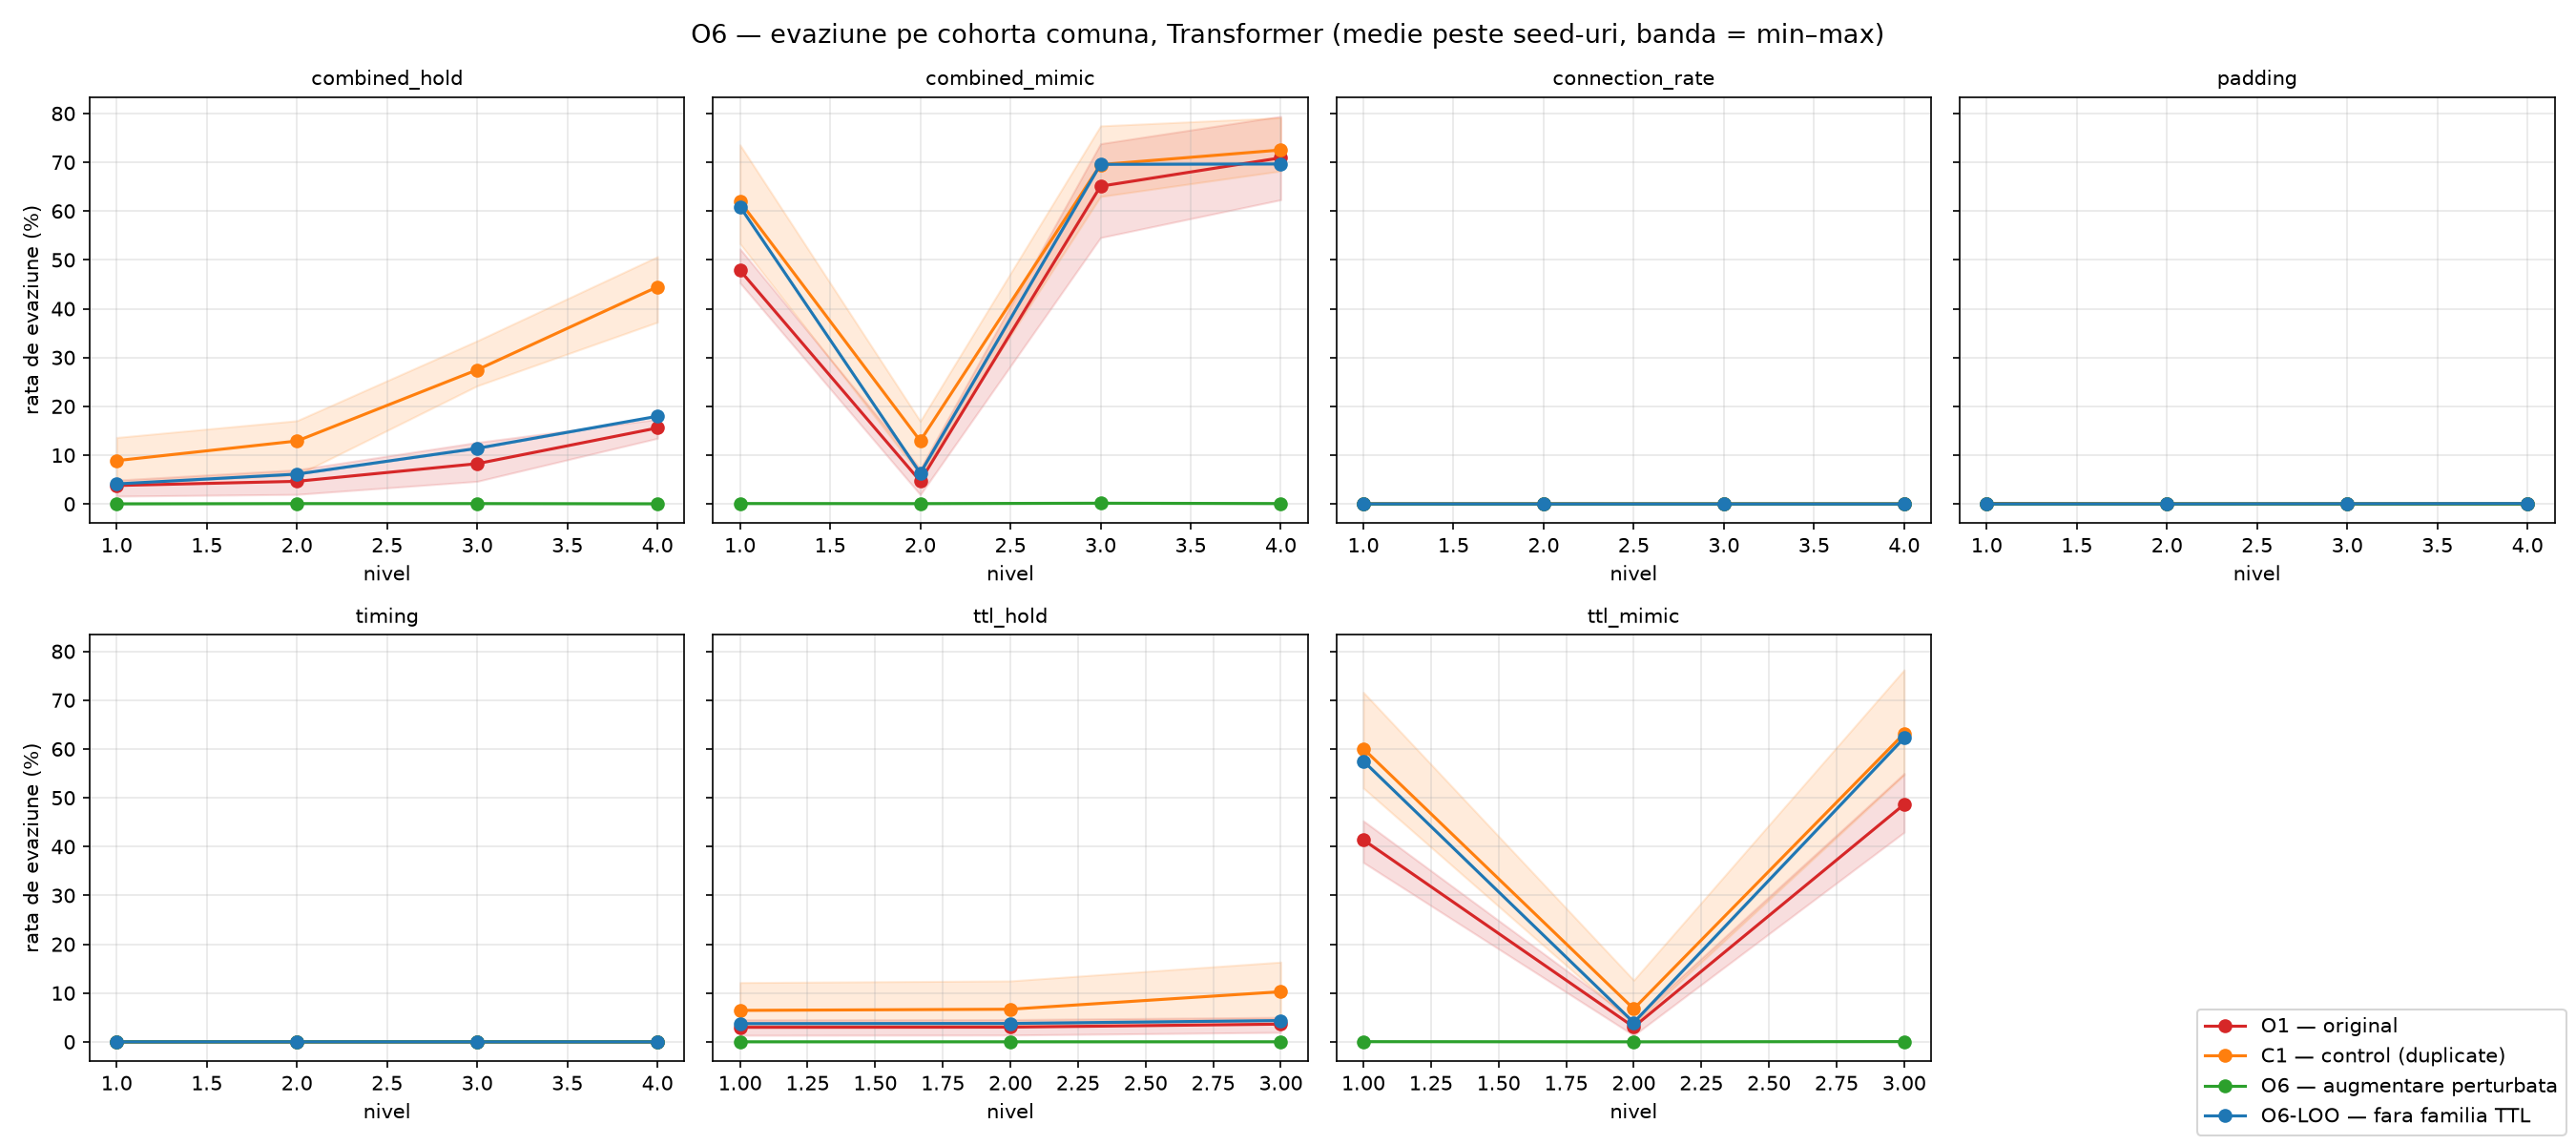
\includegraphics[width=\textwidth]{figs/o6_evasion_curves_transformer.png}
    \caption{Rata de evaziune pe mulțimea comună, per familie de transformări și nivel, pentru Transformer. Banda indică intervalul dintre repetări. Grupul antrenat fără familia TTL urmărește îndeaproape grupul de control tocmai pe transformările pe care nu le-a văzut.}
    \label{fig:o6-curbe}
\end{figure}

Două observații privind grupul de control. Prima: pentru Transformer, adăugarea de copii \emph{neperturbate} a înrăutățit situația, evaziunea crescând de la 70,92\,\% la 72,52\,\%, iar pe varianta \verb|ttl_mimic_L1| de la 41,39\,\% la 60,07\,\%. Dacă rezultatul ar fi fost raportat prin comparație directă cu grupul de referință, o parte din câștigul atribuit perturbării ar fi fost, de fapt, repararea unei degradări produse de volumul suplimentar de date. A doua: abaterea standard între repetări este de 8,55 puncte procentuale pentru grupul de referință al modelului Transformer și sub 0,08 pentru toate grupurile apărate. Antrenarea adversarială nu doar coboară rata, ci elimină și variabilitatea ei între repetări.

\subsection{Natura rezultatului: invarianță, nu alarmă permanentă}\label{subsec:o6-compozitie}

O reducere de la 96,90\,\% la 0,00\,\% ridică în mod firesc suspiciunea că modelul a învățat să declare atac pentru orice intrare, ceea ce ar elimina evaziunea distrugând utilitatea sistemului. Defalcarea celor trei rezultate posibile, prezentată în tabelul~\ref{tab:o6-compozitie}, arată că nu aceasta este explicația.

\begin{table}[!ht]
    \caption{Compoziția rezultatelor la varianta cea mai agresivă (\texttt{combined\_mimic}, nivel 4), pe mulțimea comună}
    \centering
    \begin{tabular}{|l|l|c|c|c|}
        \hline
        \textbf{Model} & \textbf{Grup} & \textbf{Corect} & \textbf{Alt tip de atac} & \textbf{Evadat} \\
        \hline
        Random Forest       & O1 & 14,80\,\% & 4,88\,\%  & 80,32\,\% \\
        \hline
        Random Forest       & O6 & \textbf{75,82\,\%} & 24,00\,\% & \textbf{0,18\,\%} \\
        \hline
        XGBoost & O1 & 0,13\,\%  & 2,97\,\%  & 96,90\,\% \\
        \hline
        XGBoost & O6 & \textbf{77,15\,\%} & 22,85\,\% & \textbf{0,00\,\%} \\
        \hline
        Transformer       & O1 & 12,88\,\% & 16,21\,\% & 70,92\,\% \\
        \hline
        Transformer       & O6 & \textbf{67,87\,\%} & 32,04\,\% & \textbf{0,09\,\%} \\
        \hline
    \end{tabular}
    \label{tab:o6-compozitie}
\end{table}

Comparația care contează este cu proporția clasificărilor corecte pe traficul \emph{nemodificat}, măsurată pe aceeași mulțime: 75,15\,\% pentru Random Forest, 78,97\,\% pentru XGBoost și 72,69\,\% pentru rețea. Modelele apărate clasifică fluxurile puternic perturbate aproape la fel de exact ca pe cele neatinse. Transformarea a devenit, pentru ele, aproape invizibilă.

Confirmarea independentă vine de la clasa traficului legitim, unde o strategie de tip alarmă permanentă ar produce o prăbușire imediată: scorul $F1$ pe această clasă scade de la 0,7665 la 0,7522 pentru Random Forest, de la 0,8467 la 0,8308 pentru XGBoost și de la 0,7380 la 0,7348 pentru rețea.

\subsection{Costul per clasă}\label{subsec:o6-perclasa}

Metricile globale ascund însă o degradare importantă, pe care criteriul de siguranță formulat în subsecțiunea~\ref{subsec:preinregistrare} a fost construit tocmai pentru a o detecta. Tabelul~\ref{tab:o6-worms} prezintă evoluția clasei \textit{Worms}, cea mai rară din set, cu 130 de exemple la antrenare și 44 la testare.

\begin{table}[!ht]
    \caption{Scorul $F1$ pe clasa \textit{Worms}, medie peste repetări}
    \centering
    \begin{tabular}{|l|c|c|c|c|c|}
        \hline
        \textbf{Model} & \textbf{O1} & \textbf{C1} & \textbf{O6} & \textbf{O6\,--\,O1} & \textbf{O6\,--\,C1} \\
        \hline
        Random Forest       & 0,5871 & 0,5014 & 0,4604 & $-0{,}127$ & $-0{,}041$ \\
        \hline
        XGBoost & 0,4907 & 0,5974 & 0,4159 & $-0{,}075$ & $\mathbf{-0{,}182}$ \\
        \hline
        Transformer       & 0,2216 & 0,1977 & 0,0942 & $-0{,}127$ & $-0{,}104$ \\
        \hline
    \end{tabular}
    \label{tab:o6-worms}
\end{table}

Descompunerea pe cele două grupuri arată că sursa degradării diferă de la un model la altul. La Random Forest, două treimi din pierdere sunt prezente deja în grupul de control, deci provin din deplasarea proporției dintre clase, nu din perturbare. La XGBoost situația este inversă: grupul de control a \emph{îmbunătățit} clasa, iar perturbarea a costat ulterior 0,182, cea mai mare pierdere înregistrată.

Nicio altă clasă nu depășește pragul de 0,05 la niciun model. Rezultatul confirmă valoarea raportării per clasă: pierderea globală de macro-$F1$ a rețelei este de 0,022, în timp ce clasa \textit{Worms} pierde mai mult de jumătate din scorul ei.

\subsection{Generalizarea la o familie de transformări nevăzută}\label{subsec:o6-generalizare}

Rezultatele de până acum măsoară robustețea la exact familia de transformări folosită la antrenare. Ele nu pot distinge între două situații foarte diferite: un model care a învățat proprietatea care face transformările eficiente și unul care a memorat transformările înseși. Distincția se poate face doar excluzând o familie din antrenare și măsurând tocmai pe ea, procedeu anunțat printre ipotezele din secțiunea~\ref{sec:ipoteze}.

Grupul O6-LOO a fost antrenat fără nicio variantă din familia TTL, rămânând doar cu umplutura, temporizarea și reducerea contoarelor de conexiuni, apoi a fost măsurat pe familia exclusă. Rezultatele sunt prezentate în tabelul~\ref{tab:o6-loo}.

\begin{table}[!ht]
    \caption{Evaziunea pe familia TTL, exclusă complet din antrenarea grupului O6-LOO}
    \centering
    \begin{tabular}{|l|c|c|c|c|}
        \hline
        \textbf{Model} & \textbf{O1} & \textbf{C1} & \textbf{O6-LOO} & \textbf{O6} \\
        \hline
        Random Forest       & 80,32\,\% & 75,51\,\% & \textbf{11,84\,\%} & 0,18\,\% \\
        \hline
        XGBoost & 96,90\,\% & 96,24\,\% & \textbf{95,68\,\%} & 0,46\,\% \\
        \hline
        Transformer       & 70,92\,\% & 72,52\,\% & \textbf{69,65\,\%} & 0,19\,\% \\
        \hline
    \end{tabular}
    \label{tab:o6-loo}
\end{table}

Rezultatul separă net cele trei modele. Random Forest generalizează: fără să fi văzut vreodată o modificare de TTL, ea coboară de la 80,32\,\% la 11,84\,\% pe varianta combinată de nivel maxim și de la 19,60\,\% la 10,88\,\% pe \verb|ttl_mimic| de nivel 3. Invarianța învățată pe umplutură și temporizare s-a transferat unei familii pe care nu a întâlnit-o.

Celelalte două modele nu generalizează deloc. Transformer rămâne la 69,65\,\% față de 70,92\,\% în grupul de referință, iar pe varianta \verb|combined_mimic| de nivel 1 se înrăutățește, de la 47,86\,\% la 60,91\,\%. Modelul cu XGBoost coboară nesemnificativ în ansamblu, de la 96,90\,\% la 95,68\,\%, dar pe două variante devine substanțial mai vulnerabil: pe \verb|ttl_hold| de nivel 3 evaziunea crește de la 49,16\,\% la 90,72\,\%, iar pe \verb|ttl_mimic| de nivel 3 de la 49,89\,\% la 92,44\,\%. Antrenarea pe transformări care nu produceau evaziune l-a făcut mai vulnerabil la cele care o produc.

O parte din explicație ține de familiile păstrate în acest grup. Umplutura, temporizarea și reducerea contoarelor produc, la modelele de referință, rate de evaziune sub 0,2\,\%. Grupul O6-LOO a fost prin urmare antrenat pe transformări pe care modelul le trata deja corect, deci fără presiune de a deveni invariant la TTL. Faptul că Random Forest a transferat totuși invarianța este partea surprinzătoare a rezultatului.

Consecința pentru interpretare este directă și trebuie enunțată fără atenuare: cifrele apropiate de zero din tabelul~\ref{tab:o6-evaziune} demonstrează robustețe la familia de transformări \emph{cunoscută}. Pentru XGBoost și pentru Transformer, ele nu pot fi citite ca robustețe la perturbări realizabile în general, întrucât singurul test direct al acestei generalizări nu arată niciuna.

\subsection{Confruntarea cu criteriile pre-înregistrate}\label{subsec:o6-verdict}

Conform subsecțiunii~\ref{subsec:preinregistrare}, criteriile au fost fixate în fișa rulării înaintea antrenării, deci înainte ca vreun rezultat să fie cunoscut. Confruntarea este prezentată în tabelul~\ref{tab:o6-verdict}.

\begin{table}[H]
    \caption{Rezultatul față de criteriile stabilite înaintea rulării}
    \centering\footnotesize
    \begin{tabular}{|p{3.9cm}|c|c|c|}
        \hline
        \textbf{Criteriu} & \textbf{Random Forest} & \textbf{XGBoost} & \textbf{Transformer} \\
        \hline
        Robustețe: câștig $\geq 10$ pp față de C1
            & TRECUT & TRECUT & TRECUT \\
            & $+93{,}4$ & $+99{,}6$ & $+97{,}6$ \\
        \hline
        Cost curat: scădere macro-$F1 \leq 0{,}02$
            & TRECUT & PICAT & PICAT \\
            & $0{,}0192$ & $0{,}0202$ & $0{,}0222$ \\
        \hline
        Siguranță: nicio clasă sub $-0{,}05$
            & PICAT & PICAT & PICAT \\
            & $-0{,}127$ & $-0{,}075$ & $-0{,}127$ \\
        \hline
        Țintă aspirațională: $\leq 30\,\%$ absolut
            & atinsă & atinsă & atinsă \\
        \hline
    \end{tabular}
    \label{tab:o6-verdict}
\end{table}

Criteriul de robustețe este îndeplinit cu un ordin de mărime peste prag, la toate cele trei modele. Criteriul de cost este depășit la două modele, dar cu mai puțin de 0,003 în ambele cazuri, sub abaterea standard între repetări a modelului Transformer. El trebuie citit ca un rezultat marginal, nu ca un eșec clar. Criteriul de siguranță este singurul depășit substanțial, la toate modelele, și indică o limitare reală a procedurii: apărarea consolidează clasele frecvente în detrimentul celei mai rare.

Faptul că două criterii din trei nu sunt îndeplinite nu invalidează experimentul, ci confirmă că formularea lor înaintea rulării a fost utilă. Un prag stabilit după cunoașterea rezultatelor ar fi fost, cu mare probabilitate, ales astfel încât să fie satisfăcut.


\section{Validarea interfeței interactive}\label{sec:validare-ui}

Cerința de proiectare a interfeței, formulată în secțiunea~\ref{sec:implinterfata}, este ca aceasta să nu constituie o implementare paralelă a perturbării. Verificarea a fost efectuată prin compararea directă a ieșirilor: pentru șapte combinații de parametri alese astfel încât să coincidă cu niveluri din setul predefinit, variantele produse de interfață au fost comparate cu cele produse de motorul de generare.

Rezultatul a fost identitate la nivel de bit în toate cele șapte cazuri. În plus, ratele de evaziune calculate live pe un eșantion aleator urmăresc îndeaproape valorile măsurate sistematic pe setul complet, cu abateri sub două unități procentuale, diferența fiind atribuibilă eșantionării.

S-a verificat de asemenea comportamentul la combinații invalide: o configurație care încalcă o constrângere de validitate este semnalată explicit, în locul afișării unei rate de evaziune. Fără această verificare, interfața ar putea prezenta un rezultat obținut pentru un flux imposibil fizic.

\section{Sinteza rezultatelor}\label{sec:sinteza}

Rezultatele experimentale susțin ipoteza de la care pornește lucrarea, într-o formă mai puternică decât se anticipa. Se rețin șapte constatări, ultimele două privind partea de apărare.

\textbf{Prima.} Toate cele trei modele semnalează aproape fiecare atac pe trafic nemodificat, între $97{,}6\%$ și $99{,}9\%$ dintre fluxurile de atac declanșând o alarmă. Cifra nu descrie însă un detector bun, întrucât aceleași modele semnalează și între $24\%$ și $41\%$ din traficul legitim. Pentru evaluarea adversarială contează doar prima parte a acestei observații, care garantează că măsurătoarea pornește de la fluxuri efectiv detectate.

\textbf{A doua.} O singură modificare de TTL, cu cost practic nul pentru atacator și compatibilă cu păstrarea funcționalității atacului în modelul de amenințare adoptat, duce XGBoost de la $0\%$ la peste $50\%$ evaziune. Combinată cu umplutură și dilatare temporală, rata ajunge la aproape $97\%$.

\textbf{A treia.} Robustețea și acuratețea nu variază în același sens. Modelul cu cele mai bune metrici pe trafic nemodificat este și cel mai fragil sub perturbare. Performanța pe trafic nemodificat nu permite, așadar, singură, estimarea robusteței adversariale.

\textbf{A patra.} Cauza este măsurabilă, nu speculativă: modelul respectiv concentrează $54{,}6\%$ din capacitatea sa de detecție într-o singură caracteristică, trivial de modificat, care s-a dovedit a fi un artefact al mediului de captură, nu un semnal despre atac.

\textbf{A cincea.} Rezistența aparent superioară a modelului Transformer nu provine dintr-o reprezentare mai bună, ci din faptul că modelul se sprijină preponderent pe o caracteristică generată de victimă, pe care atacatorul nu o poate modifica. Doar $26{,}0\%$ din capacitatea sa de detecție este accesibilă, iar atunci când constrângerea de accesibilitate este relaxată artificial, rata sa de evaziune urcă la $71{,}1\%$.

\textbf{A șasea.} Reantrenarea pe trafic perturbat elimină aproape complet vulnerabilitatea măsurată: evaziunea în cel mai rău caz scade sub $0{,}5\%$ la toate cele trei modele, de la valori între $71\%$ și $97\%$. Rezultatul nu provine dintr-o strategie degenerată de tip alarmă permanentă, fiindcă modelele apărate clasifică fluxurile perturbate aproape la fel de exact ca pe cele neatinse, și rămâne valabil față de grupul de control, care izolează efectul volumului suplimentar de date. Costul este o scădere de macro-$F1$ sub $0{,}023$ și o degradare substanțială a clasei celei mai rare.

\textbf{A șaptea.} Această robustețe nu se transferă însă la transformări nevăzute, decât pentru un singur model. Antrenat fără nicio variantă din familia TTL și măsurat tocmai pe ea, Random Forest coboară de la $80{,}3\%$ la $11{,}8\%$, în timp ce XGBoost și Transformer rămân practic neschimbate, la $95{,}7\%$ și respectiv $69{,}7\%$.

Ultima constatare merită subliniată, întrucât ea nuanțează o concluzie care altfel ar fi fost formulată greșit: ceea ce s-ar fi putut raporta drept robustețe arhitecturală este, în realitate, o consecință a unei particularități a datelor. O evaluare care ar fi comparat doar ratele de evaziune, fără analiza de sensibilitate, ar fi condus la recomandarea eronată de a prefera această arhitectură pentru robustețea ei. Aceeași observație se aplică, simetric, ultimei constatări: valorile apropiate de zero din tabelul~\ref{tab:o6-evaziune} ar fi putut fi raportate ca robustețe generală dacă grupul de generalizare nu ar fi fost inclus în experiment.
